\documentclass{article}

\usepackage[main, final]{neurips_2026}

\usepackage[utf8]{inputenc} % allow utf-8 input
\usepackage[T1]{fontenc}    % use 8-bit T1 fonts
\usepackage{hyperref}       % hyperlinks
\usepackage{url}            % simple URL typesetting
\usepackage{booktabs}       % professional-quality tables
\usepackage{amsfonts}       % blackboard math symbols
\usepackage{nicefrac}       % compact symbols for 1/2, etc.
\usepackage{microtype}      % microtypography
\usepackage{xcolor}         % colors
\usepackage{float}
\usepackage{graphicx}
\usepackage{subcaption}
\usepackage{natbib}

\title{Venturing into the (W)OODs: An Exploration Beyond IID Scenarios}

\author{
  Faaiz Khan \\
  Syed Babar Ali School of Science and Engineering\\
  Lahore University of Management Sciences\\
  Lahore, Pakistan\\
  \texttt{25280051@lums.edu.pk} \\
}

\begin{document}

\maketitle

\begin{abstract}
  Standard supervised learning relies heavily on the assumption that training and test data are drawn from the same probability distribution and share identical label spaces. However, these independent and identically distributed (IID) assumptions are frequently violated in real-world deployment, where models may encounter visual shifts and new domains with novel classes. This paper presents a systematic empirical evaluation of model robustness across four non-IID scenarios: inductive biases, unsupervised domain adaptation, domain generalization, and open-set recognition. We first evaluate convolutional, transformer-based, and contrastive architectures under controlled shape, texture, color, and spatial interventions to investigate the relationship between prediction stability and representation stability. We then explore unsupervised domain adaptation using marginal and class-conditional alignment strategies (DAN, DANN, CDAN), examining whether reducing domain discrepancy effectively preserves class separation or inadvertently induces negative transfer. By strictly restricting target domain access, we also evaluate domain generalization to compare explicit source-domain feature alignment against the local parameter stability enforced by Sharpness-Aware Minimization (SAM). Finally, we tackle open-set recognition to test the assumption that higher closed-set accuracy inherently improves open-set rejection. By contrasting post-hoc novelty scores with placeholder learning (PROSER) and RPL, we aim to expose how models manage the distinct challenges of near-semantic versus far-semantic anomalies. You may find the associated code and \LaTeX files for this assignment in the following GitHub repository: \url{https://github.com/FaaizKhan1999/atml-assignment1}
\end{abstract}

\section{Introduction}

Deep models achieve remarkable accuracy under closed-set, IID scenarios and evaluation protocols. However, this performance frequently degrades upon real-world deployment. A model may achieve strong in-distribution metrics by relying on statistical regularities that do not remain stable across different environments: specific textures, backgrounds, positional cues, etc. Consequently, an object from a known class might appear in a novel style, test data may arrive from an entirely unseen domain, or an input might belong to a semantic category absent from the training set entirely.

At present, these distribution shifts are often treated as isolated phenomena. While certain techniques do attempt to bridge these gaps, simply minimizing statistical discrepancy between source and target domains does not necessarily preserve class-discriminative information, and models achieving high closed-set accuracy frequently fail to reject anomalous inputs when tested in open-set conditions. There is a critical need to jointly evaluate how inductive biases, feature alignment, and optimization strategies interact with a network's ability to maintain its representational power.

This work addresses this gap through a unified empirical framework that connects observed out-of-distribution performance to the underlying representations, architectures, and training objectives. We structure our exploration across four escalating relaxations of the IID assumption. First, we isolate the visual dependencies of ResNet, Vision Transformer (ViT), and CLIP backbones using controlled cue-conflict and spatial-permutation interventions. Second, we explore unsupervised domain adaptation, testing if explicit feature alignment (DAN) and adversarial confusion (DANN, CDAN) can successfully utilize unlabeled target data without corrupting semantic structure. Third, we strictly remove target-domain access to study domain generalization, comparing the efficacy of empirical risk minimization against source-domain feature alignment and Sharpness-Aware Minimization (SAM). Finally, we abandon the closed-set assumption entirely to evaluate how models identify and reject inputs from unknown classes. 

By synthesizing across these dimensions, this paper answers the following unifying questions: what information should a robust representation preserve, what variations must it suppress, and when should a model reject an input rather than force a confident prediction? 

\section{Inductive Biases and Feature Representations}
\label{section:biases}

An inductive bias represents a set of assumptions introduced by a model's architecture, training data, or objective function to prioritize certain solutions over others. For small models, these biases generally fall into two interconnected categories: structural and semantic. Structural biases encompass mathematical priors, such as the spatial locality and translation equivariance enforced by convolutions, or the global routing and permutation invariance of self-attention. These structural constraints, in turn, heavily influence a model's semantic biases, dictating whether it prioritizes visual primitives like shape, texture, background, or color when establishing decision boundaries.

These biases ultimately govern the formation of the model's feature representation: the latent vector extracted immediately prior to the final classification head. Because the raw input dimension is vastly larger than this latent bottleneck, the network is forced to compress information and learn the underlying data manifold. This dimensionality reduction projects high-dimensional pixel inputs into a dense, lower-dimensional semantic space, mapping features such that their geometry reflects conceptual similarities rather than raw spatial overlap.

\subsection{Methodology}

\paragraph{Datasets and Models}

We empirically evaluate our hypotheses using the STL-10 dataset. We extract latent feature representations from three frozen, pre-trained network backbones: a 50-layer Residual Network (ResNet-50), a Vision Transformer (ViT-B/16), and a Contrastive Language-Image Pretraining (CLIP) ViT-B-32 model. The evaluated representations consist of the global-average-pooled feature for the ResNet, the final class token for the ViT, and the normalized image embedding for CLIP. The CLIP model is additionally evaluated in a zero-shot capacity utilizing a fixed prompt template. An overview of the training process including optimization hyperparameters and the training and validation accuracy trajectories are provided in Appendix \ref{appendix:task1_training}.

\paragraph{Intervention Design}

To ensure a standardized and controlled evaluation, we sample a class-balanced subset of 500 test images. All interventions are constructed on a common $224 \times 224$ RGB canvas prior to applying model-specific normalizations. After establishing a clean baseline by recording top-1 accuracy, macro-F1 score, and mean maximum confidence, we systematically apply four distinct visual interventions. First, to isolate the effect of chromatic information removal, images are converted to grayscale, followed by a hue rotation as a secondary transformation to assess model sensitivity to altered color statistics while strictly preserving object geometry. Second, we evaluate shape versus texture bias by generating cue-conflict images using Adaptive Instance Normalization \citep{Huang_2017_ICCV}, combining the content (shape) of one class with the style (texture) of another. We select five unordered class pairs and generate stylizations in both directions, yielding over 200 valid conflict images after applying a rigorous visual rejection rule to discard failed stylizations. For this intervention, shape bias is computed based solely on predictions matching either the intended shape or texture label. Third, to evaluate spatial sensitivity and translation equivariance, each image is translated by 0, 8, 16, and 32 pixels across all four cardinal directions using reflection padding and shifted crops, and the results are averaged to compute prediction consistency as a function of displacement. Finally, we disrupt the global structural organization of the image while retaining local pixel evidence by partitioning each image into a $4 \times 4$ spatial grid and applying a fixed, non-identity patch permutation.

\paragraph{Representation Stability Analysis}

To investigate whether the underlying feature space shifts independently of the final classifier output, we pair each transformed image with its clean counterpart and compute the cosine stability of the extracted latent features. Finally, we fit a single two-dimensional t-SNE projection to the combined clean and transformed features for each respective backbone. This allows for a visual analysis of class separation, condition mixing, and the identification of specific transformations that displace examples from their original clean clusters.

\subsection{Results and Analysis}

\paragraph{Semantic Biases: Color Sensitivity and Cue Conflicts}

Figure~\ref{fig:task1_performance_shape} summarizes the classification performance across the clean baseline, color interventions, and spatial perturbations, alongside the computed shape bias metrics. The models exhibit minimal reliance on chromatic information; grayscale conversion and hue rotation induce negligible accuracy degradation (ranging from a 1.6\% drop for ResNet to a 4.6\% drop for ViT). 

Under cue-conflict evaluations, all backbones demonstrate a structural preference for global shape over local texture, though the magnitude varies. This contradicts the findings of \cite{geirhos2022imagenettrainedcnnsbiasedtexture} which asserts that CNNs are texture-biased. We hypothesize that the reason for this is our usage of STL-10 with AdaIN style transfer whereas \cite{geirhos2022imagenettrainedcnnsbiasedtexture} use ImageNet with a highly stylized style transfer. Having said that, ResNet-50 exhibits the weakest shape bias (90.3\%), somewhat reflecting the localized nature of convolutional feature extraction. This vulnerability is evident in Figure~\ref{fig:task1_cue_conflicts}, where ResNet occasionally classifies based on texture, whereas ViT (94.1\%) and CLIP (95.2\%) prioritize the underlying shape. While the employed style transfer destroys semantic meaning in roughly 20\% of the candidate images, the retained coverage (~75.8\% to 82.7\%) provides a statistically robust pool of valid decisions, firmly validating the dominance of shape bias across these architectures.

\begin{figure}[ht]
  \centering
  \begin{minipage}{0.48\textwidth}
    \centering
    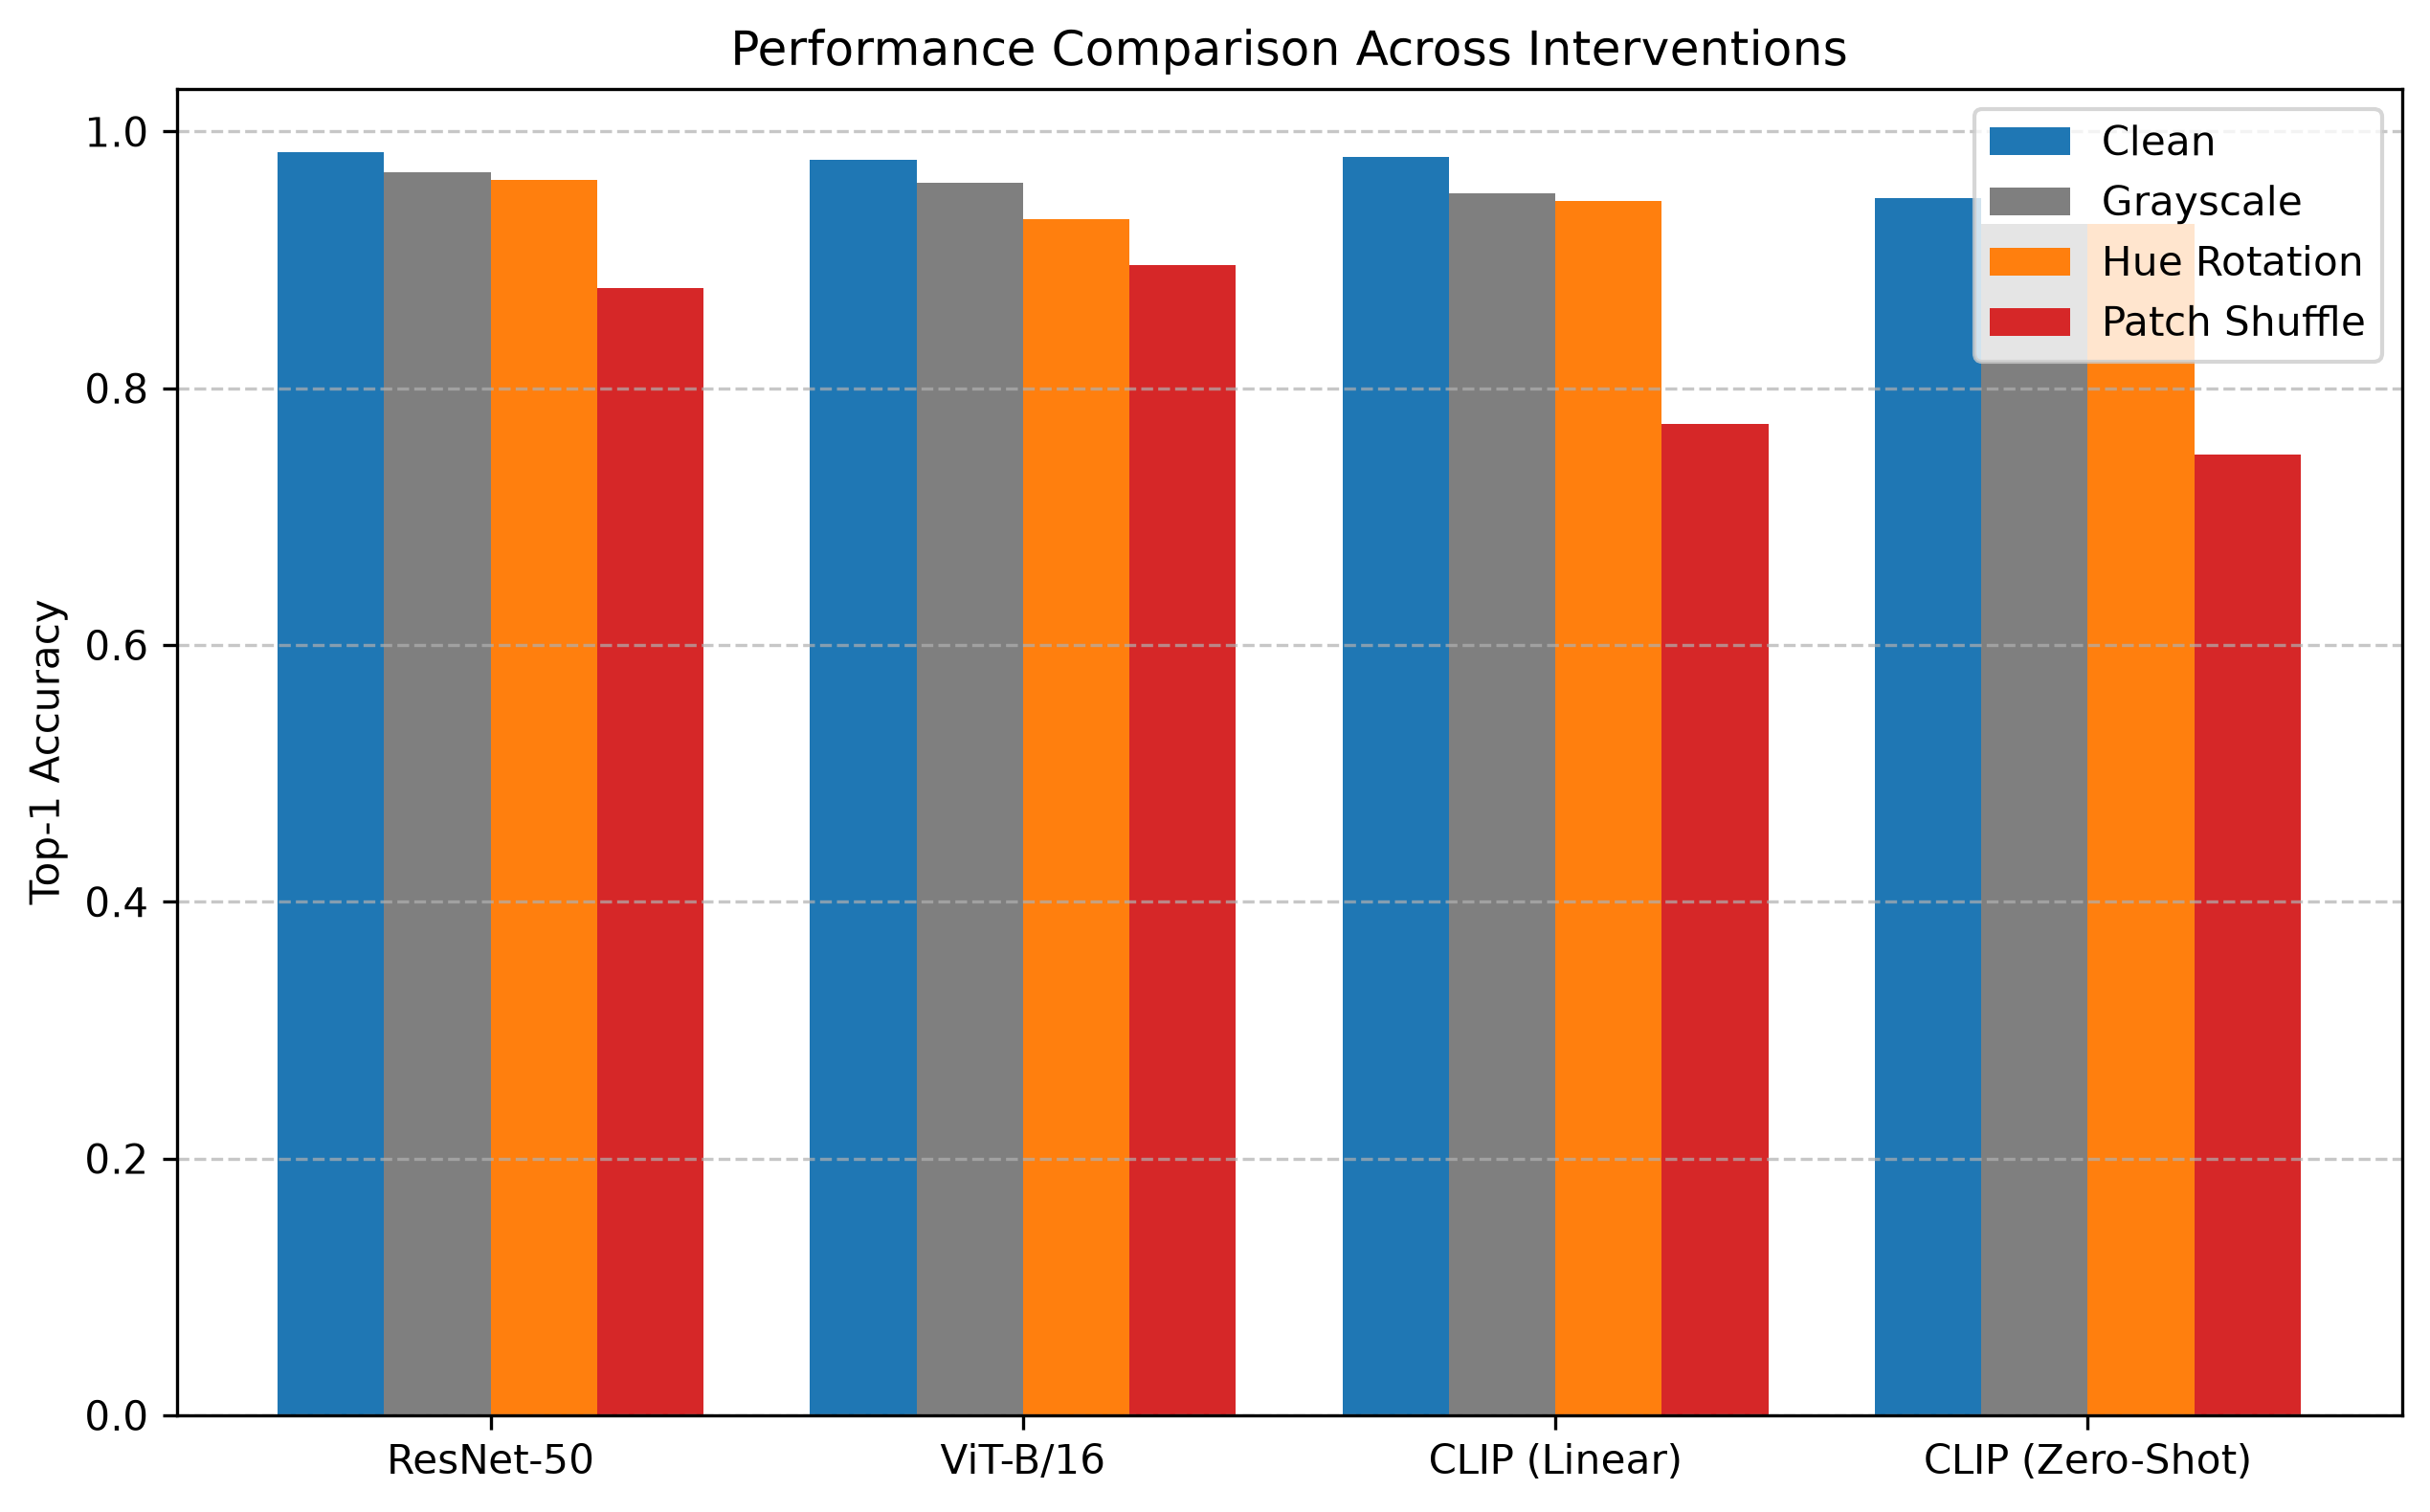
\includegraphics[scale=0.3]{../task1/results/performance_comparison.png}
  \end{minipage}\hfill
  \begin{minipage}{0.48\textwidth}
    \centering
    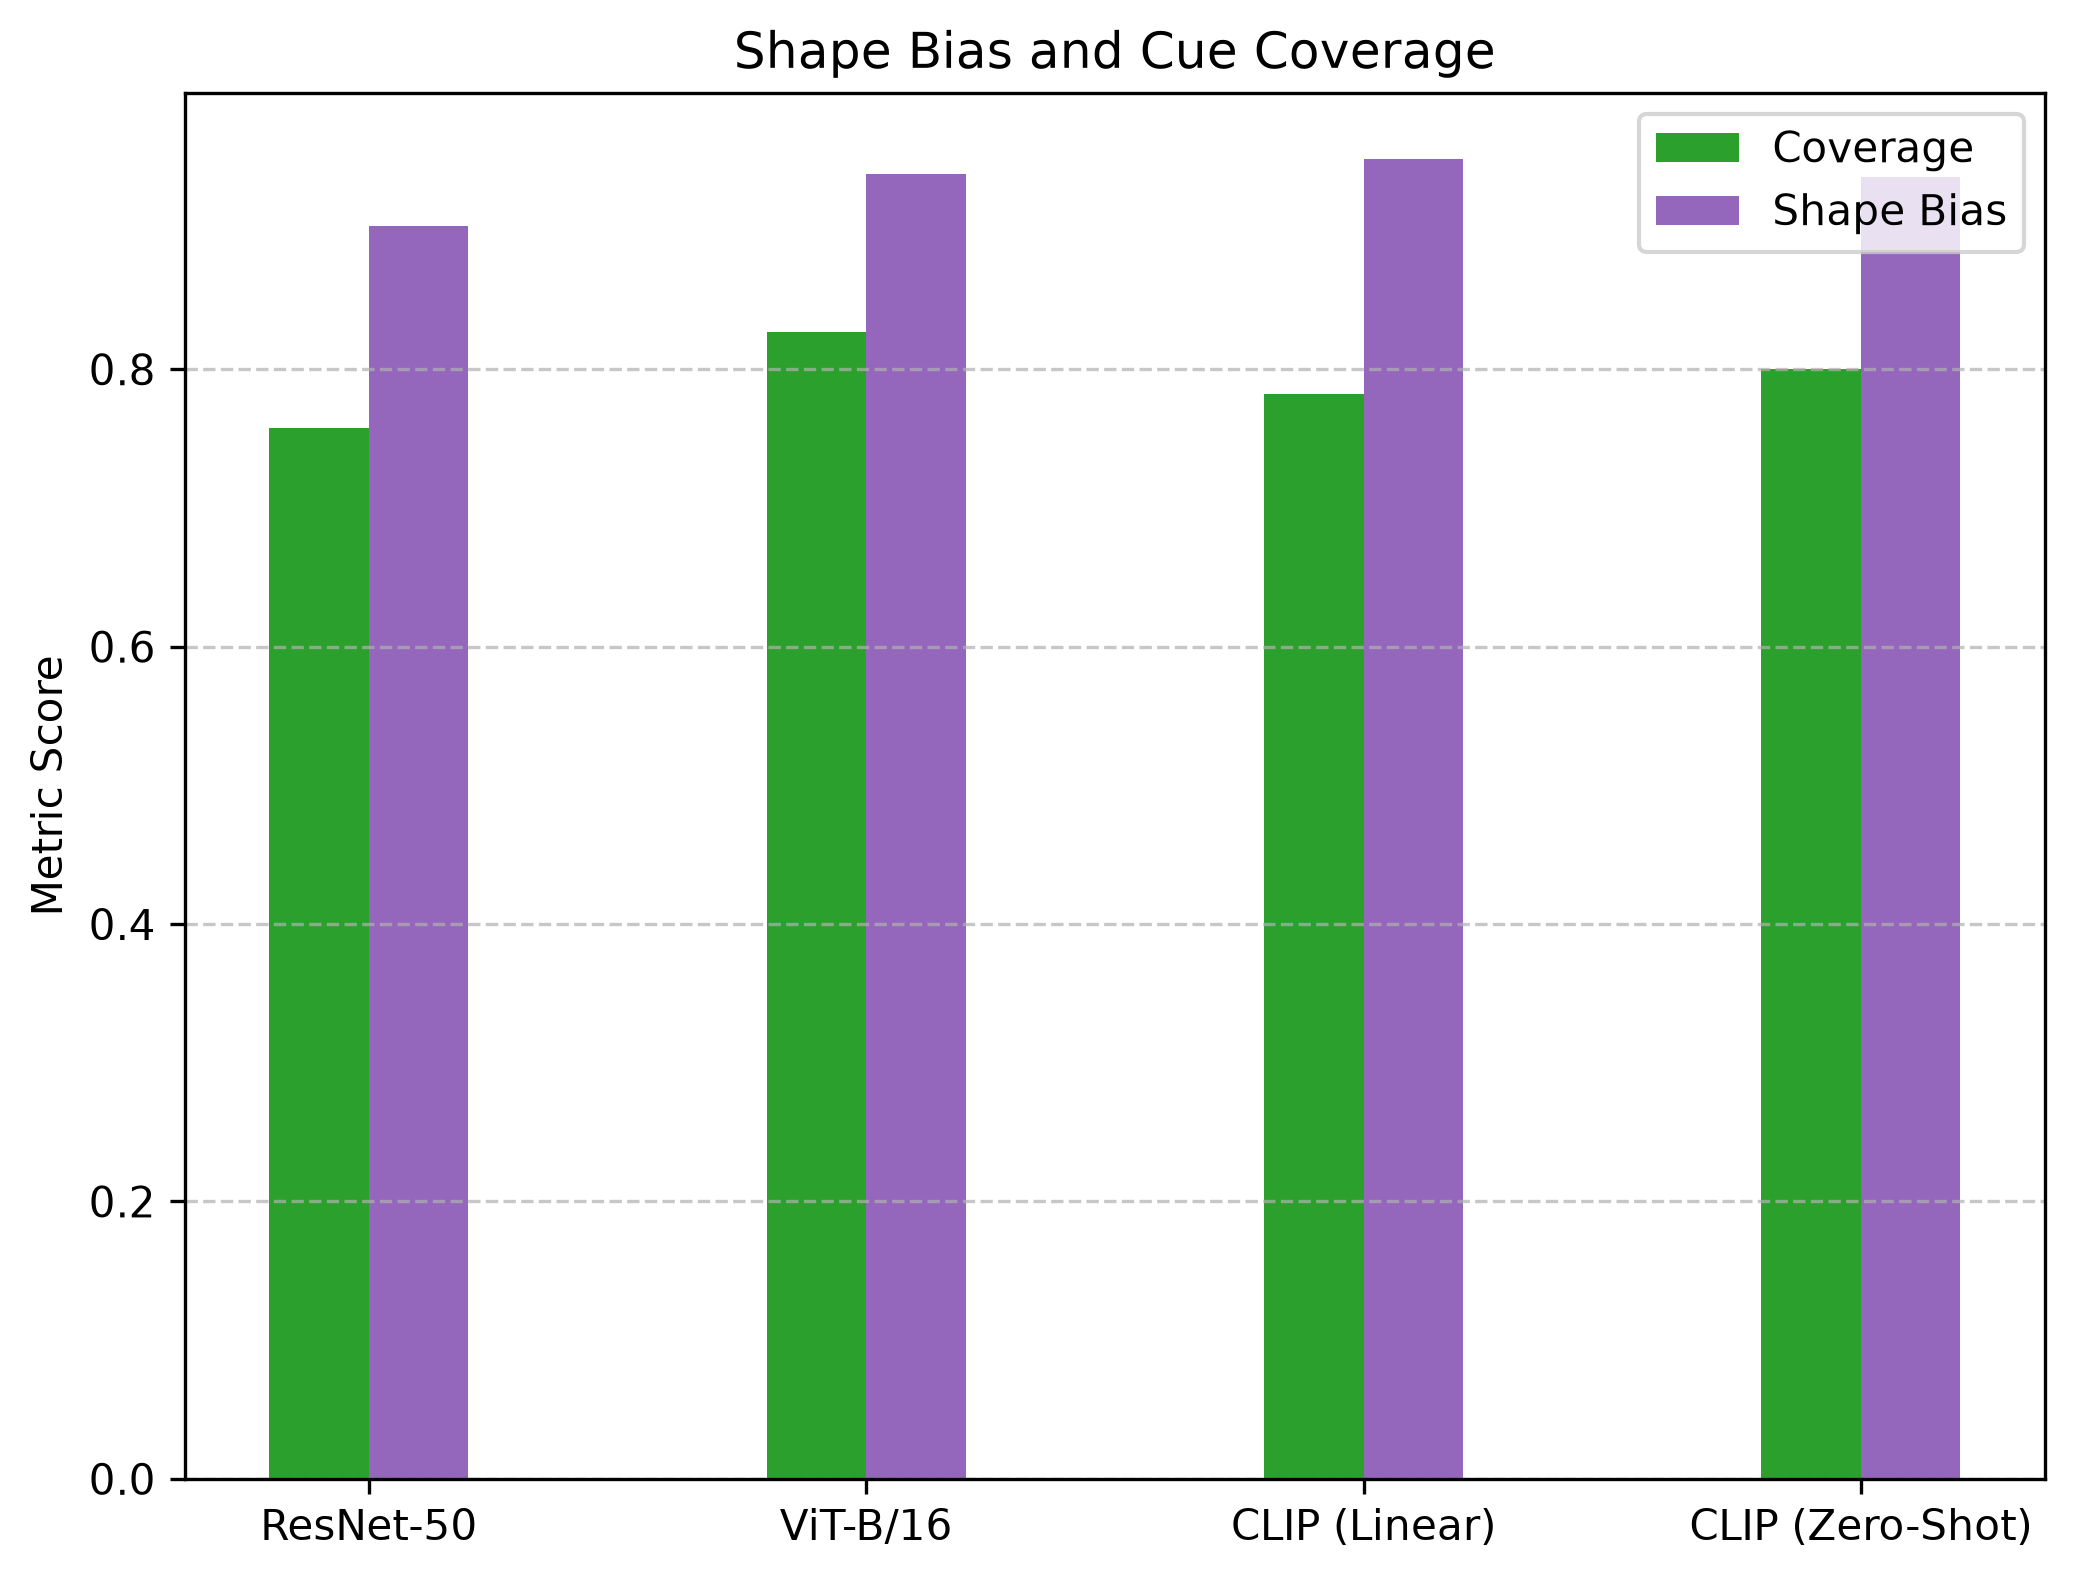
\includegraphics[scale=0.3]{../task1/results/shape_bias_summary.png}
  \end{minipage}
  \caption{Impact of controlled interventions on model accuracy (left) and extracted shape bias and coverage metrics (right). The models remain robust to color variations and predominantly favor shape cues over texture across all backbones.}
  \label{fig:task1_performance_shape}
\end{figure}

\begin{figure}[ht]
  \centering
  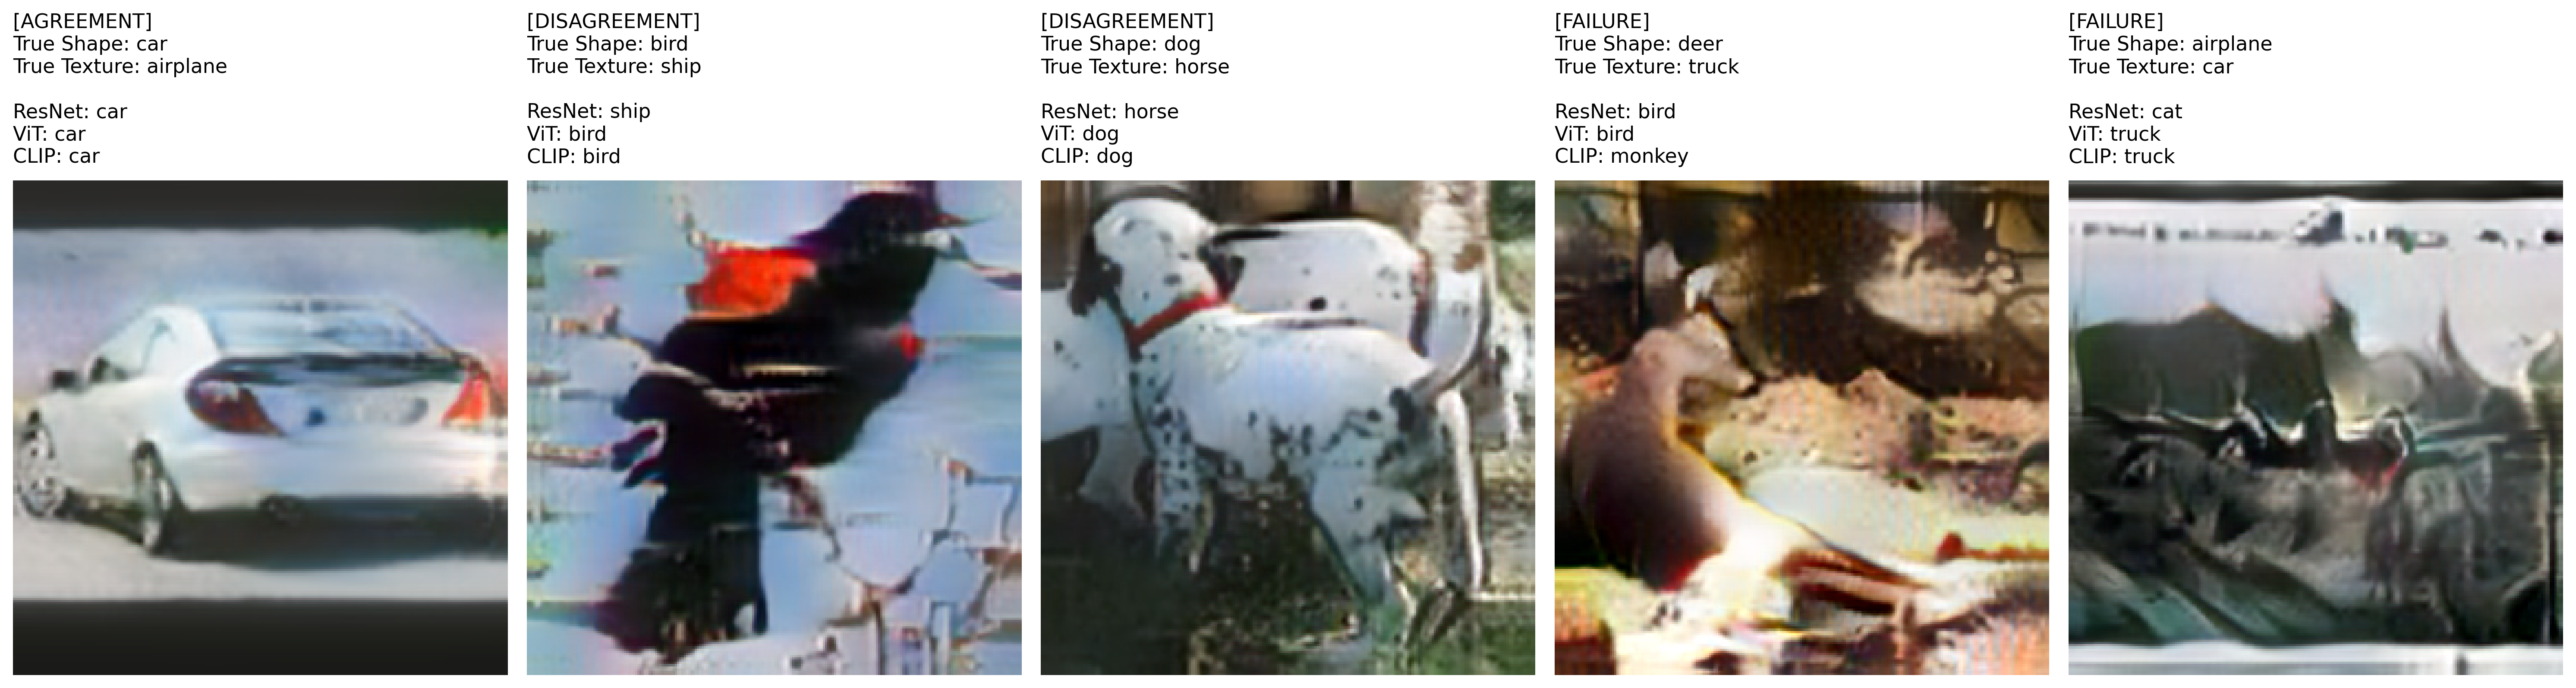
\includegraphics[width=0.8\textwidth]{../task1/results/cue_conflict_visuals.png}
  \caption{Selected cue-conflict images highlighting model agreements, disagreements, and texture-based failures. ResNet occasionally defaults to texture, while ViT and CLIP consistently track the underlying shape semantics.}
  \label{fig:task1_cue_conflicts}
\end{figure}

\paragraph{Structural Biases: Spatial Locality and Translation}
Figure~\ref{fig:task1_translation} illustrates model prediction consistency as a function of spatial displacement. All models demonstrate exceptional translation invariance, with accuracy dropping less than 2\% at the maximum displacement ($\delta=32$). Notably, ViT achieves the highest positional independence (99.0\% consistency), suggesting that global self-attention mechanisms are inherently less position-sensitive than their convolutional counterparts, aligning with the idea in \cite{NEURIPS2021_652cf383} that Vision Transformers successfully aggregate global context much earlier in the network than CNNs.

However, Figure~\ref{fig:task1_performance_shape} also shows that disrupting global spatial organization via patch shuffling exposes stark differences in local evidence aggregation. Both ResNet and ViT suffer only moderate accuracy drops with ViT performing the best, indicating an ability to function as classifiers that aggregate local evidence. Conversely, CLIP suffers a severe 19.8\% accuracy drop. This architectural divergence highlights the impact of pretraining: while ImageNet classification encourages models to lock onto local discriminative features, CLIP's contrastive language-image pretraining requires holistic global organization to successfully align with language semantics.

\begin{figure}[ht]
  \centering
  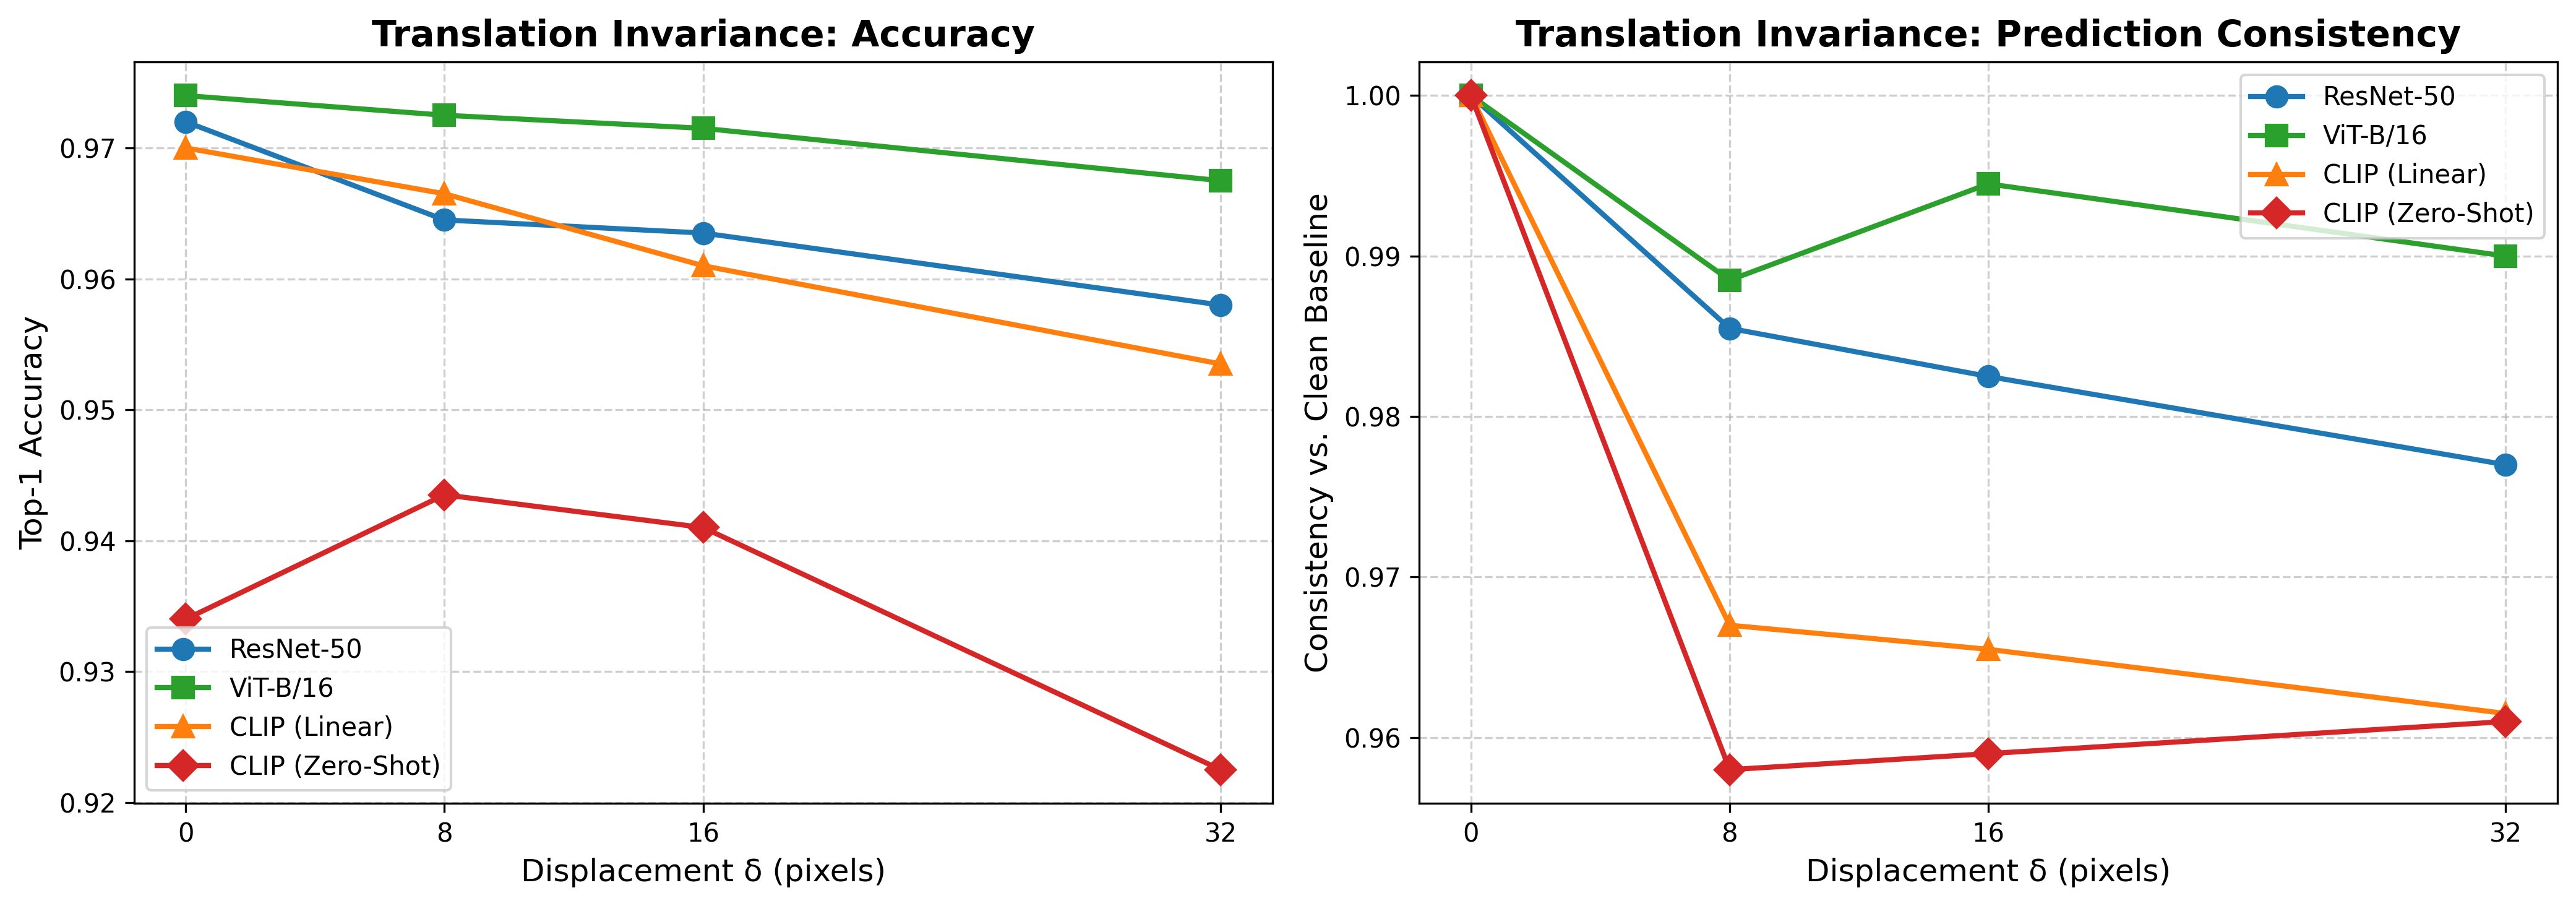
\includegraphics[width=0.6\textwidth]{../task1/results/translation_plot.png}
  \caption{Prediction consistency against spatial translation displacement ($\delta \in \{0, 8, 16, 32\}$ pixels). All architectures maintain high stability under spatial shifts, with ViT demonstrating near-perfect translation invariance.}
  \label{fig:task1_translation}
\end{figure}

\paragraph{Prediction vs. Representation Stability}
When subjected to translation and grayscaling, the models exhibit robust prediction and representation stability, with transformed feature embeddings clustering tightly around the clean distributions (see Appendix~\ref{appendix:tsne} for full t-SNE visualizations; Figure~\ref{fig:task1_rep_stability} quantifies cosine stability).

Under cue conflicts, the ImageNet-trained models exhibit a profound mismatch between prediction and feature stability. While ResNet and ViT maintain stable predictions ($>90\%$ shape bias), their underlying representations shift drastically, dropping to cosine stabilities of approximately 0.47. This suggests the models extract substantially altered features when style changes, yet the linear classifier successfully maps these displaced embeddings to the correct semantic class.

In contrast, CLIP demonstrates strong alignment between its latent representations and final predictions. Its features remain remarkably stable under cue-conflict (cosine stability of 0.79), echoing its high shape bias. Furthermore, CLIP's zero-shot behavior almost perfectly mirrors its trained linear head, with both exhibiting roughly 95\% shape bias and suffering massive degradation under patch shuffling. This definitively confirms that these inductive biases are deeply embedded within the frozen pretrained representations rather than being acquired by the downstream classifier head.

Crucially, patch shuffling exposes a revealing tension between absolute angles (cosine similarity) and relative class separation for CLIP. Because patch shuffling feeds the network the exact same visual tokens in a scrambled order, the raw ingredients remain unchanged, which keeps the absolute cosine similarity relatively high. However, destroying the spatial coherence strips away the global context needed to actually distinguish between classes. As a result, the scrambled patch representations collapse into a single, isolated cluster. They group together because they have all become similarly meaningless noise, confirming that high feature stability does not guarantee class discriminability.

\begin{figure}[ht]
  \centering
  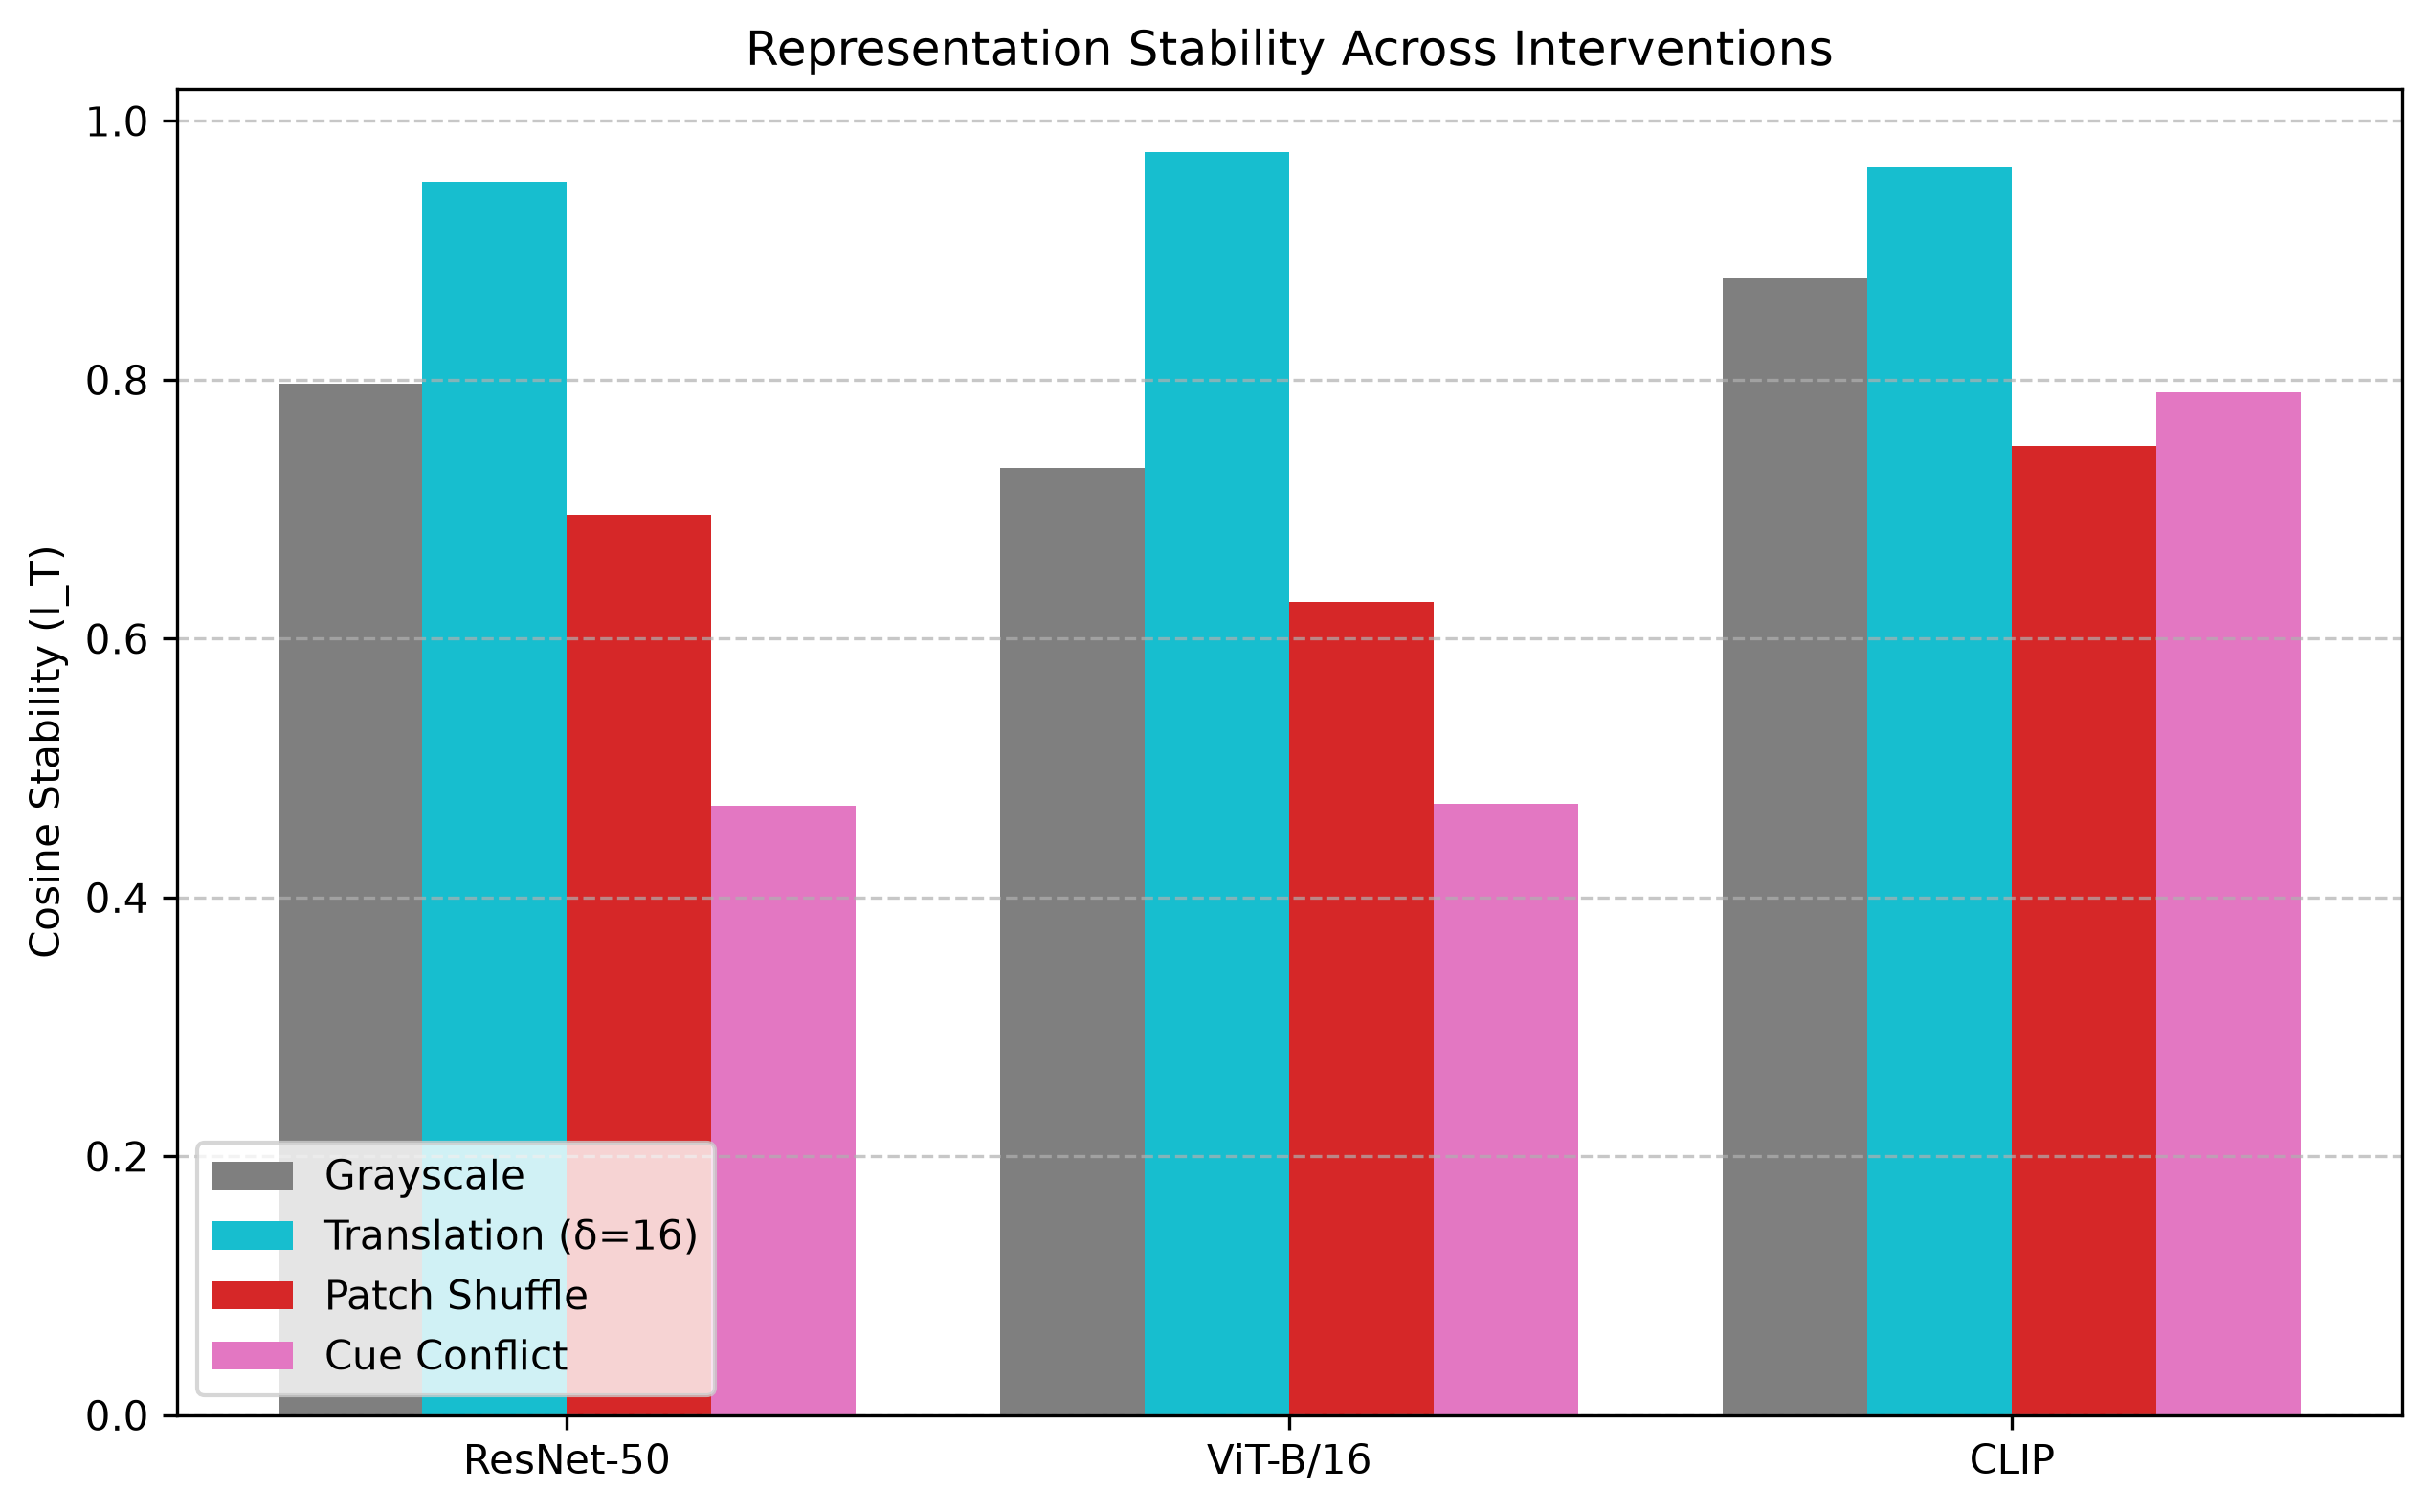
\includegraphics[scale=0.3]{../task1/results/representation_stability_summary.png}
  \caption{Analysis of feature-level cosine stability across models when subjected to varying visual interventions. ImageNet models experience severe representation drift under cue conflicts despite stable predictions, while CLIP maintains high angular stability.}
  \label{fig:task1_rep_stability}
\end{figure}

\section{Unsupervised Domain Adaptation}
\label{section:uda}

In unsupervised domain adaptation (UDA), a model is provided with labeled examples from one or more source domains and unlabeled examples from a target domain during training. While all domains share an identical class space, their underlying visual distributions differ significantly. The primary objective is to use the unlabeled target structure to minimize this domain gap, improving target recognition without degrading the discriminative class information learned from the source domains.

\subsection{Methodology}

\paragraph{Dataset and UDA Protocol}
We conduct our adaptation experiments utilizing the PACS dataset, which comprises seven object categories distributed across four distinct visual domains. Following the UDA protocol, we designate Sketch as the completely unlabeled target domain and utilize Photo, Art Painting, and Cartoon as the labeled source domains.

\paragraph{Architecture and Optimization}
We employ a pre-trained ResNet-18 backbone, replacing the ImageNet classification layer with a randomly initialized seven-class linear head. Each training iteration processes a perfectly balanced batch comprising 24 source examples (eight per domain) and 24 unlabeled target examples. 

\paragraph{Alignment Strategies}
We evaluate four progressive adaptation paradigms. The Source-only ERM baseline is optimized exclusively on labeled source data using standard cross-entropy, establishing the unadapted transferability of the network. DAN \citep{pmlr-v37-long15} introduces marginal alignment by applying a Maximum Mean Discrepancy (MMD) penalty to the 512-dimensional feature space prior to the classifier head. We compute this discrepancy using a sum of three Radial Basis Function (RBF) kernels with bandwidths scaled to 0.5, 1, and 2 times the median pairwise squared feature distance. DANN \citep{JMLR:v17:15-239} replaces the explicit MMD penalty with a binary domain discriminator (featuring a 256-unit hidden layer, ReLU activation, and 50\% dropout) optimized via a gradient-reversal layer. We employ a standard progressive scaling schedule for the reversed gradients to allow initial task learning before enforcing domain confusion. Lastly, CDAN \citep{NEURIPS2018_ab88b157} executes class-conditional alignment by feeding the discriminator the flattened outer product of the latent feature vector and the classifier's probability vector. An overview of the training process including optimization hyperparameters and the training and validation accuracy trajectories are provided in Appendix \ref{appendix:task2_training}.


\paragraph{Diagnostics and Controlled Study}
To independently quantify the amount of domain-specific information retained by each model, we compute a domain separability score. We freeze the adapted backbones, extract representations from a balanced 70/30 split of combined source-validation and target images, and train a logistic regression classifier ($C=1$) to distinguish source features from target features. Held-out accuracy on this task serves as our separability metric, where chance performance (50\%) indicates perfect domain confusion. Finally, for our controlled design study, we systematically vary the maximum gradient-reversal strength in the DANN architecture over the set $\{0.25, 0.5, 1\}$ while retaining the standard progressive scheduling. This isolates the impact of alignment pressure on source performance, domain separability, and target recognition.

\subsection{Results and Analysis}

\paragraph{The Unadapted Domain Gap and Baseline Performance}
Table~\ref{tab:task2_performance} presents the aggregate classification metrics for all adaptation strategies across the source validation domains and the unseen Sketch target domain. The Source-Only empirical risk minimization baseline achieves a robust mean source macro-F1 of 93.89\%, performing consistently well across Photo (95.77\%), Art Painting (90.63\%), and Cartoon (95.26\%). However, transferring this model to the Sketch domain exposes a severe visual distribution gap, with target accuracy plummeting to 57.52\%. A class-level analysis (Table~\ref{tab:task2_per_class}) reveals that this performance degradation is not uniformly distributed. The unadapted model struggles significantly with specific semantic categories, particularly 'horse' (39.2\% accuracy), 'elephant' (47.6\%), and 'guitar' (50.3\%), indicating an over-reliance on source-specific textures or backgrounds for these objects.

\paragraph{Invariance vs. Discriminability: Marginal Alignment}
UDA frameworks work on the assumption that reducing domain separability inherently translates to improved target recognition. The marginal alignment experiments directly contradict this assumption. As shown in Table~\ref{tab:task2_performance}, DAN successfully achieves near-perfect domain confusion, dropping the domain separability score to 53.14\% (approaching random chance). However, this statistical invariance is accompanied by catastrophic negative transfer, yielding a target accuracy of just 2.04\%. Similarly, DANN under baseline hyperparameters collapses entirely (4.35\% target accuracy) with 100\% domain separability. This proves that marginal feature alignment can easily achieve low statistical discrepancy by destroying the underlying class boundaries, rendering the representations domain-invariant but semantically useless, a theoretical vulnerability formally established by \citet{pmlr-v97-zhao19a}.

\paragraph{Preserving Semantic Structure: Class-Conditional Alignment}
In contrast to the catastrophic failures of marginal alignment, class-conditional alignment successfully bridges the domain gap without erasing class features. CDAN achieves the highest target recognition (68.03\%, a +10.51\% improvement over the baseline) despite maintaining a high domain separability score of 99.86\%. By conditioning the domain discriminator on the classifier's probability predictions, CDAN enforces alignment between semantically corresponding regions across domains rather than forcing naive global distribution matching. However, aggregate improvements mask class-specific negative transfer. While CDAN produces massive positive transfer for previously underperforming classes like 'horse' (+41.2\%) and 'guitar' (+33.4\%), it simultaneously induces severe negative transfer on 'person' (-45.0\%) and 'dog' (-34.5\%). This highlights a critical limitation that even conditional alignment can inappropriately conflate semantically adjacent feature boundaries if target domains lack definitive structural cues.

\paragraph{Controlled Study: The Alignment Trade-off}
Figure~\ref{fig:task2_controlled} details the controlled study evaluating the impact of increasing the maximum Gradient Reversal Layer (GRL) strength in the DANN architecture. The results reveal a sharp optimization trade-off. At a reduced GRL strength of 0.25, DANN effectively adapts, yielding a target accuracy of 65.31\% while maintaining a high source F1 of 91.38\%. However, as alignment pressure increases to 0.5 and 1.0, the model triggers sudden feature collapse, plummeting target accuracy to 19.45\% and 4.35\%, respectively. Crucially, the optimal setting ($\alpha_{max}=0.25$) could have been selected reliably without violating the transductive UDA protocol; it is the sole configuration that preserved the mean source-validation macro-F1 score, confirming that source-side stability acts as a robust proxy for target performance when tuning hyperparameter constraints.

\begin{table}[ht]
  \caption{Task 2 main evaluation metrics across source domains and target (Sketch) domain. While marginal alignment methods (DAN, DANN) suffer catastrophic negative transfer, class-conditional alignment (CDAN) successfully improves target accuracy despite maintaining high domain separability.}
  \label{tab:task2_performance}
  \centering
  \setlength{\tabcolsep}{4.5pt} 
  \begin{tabular}{lcccccccc}
    \toprule
    Method & Photo & Art & Cartoon & Mean Src & Tgt Acc & Tgt F1 & $\Delta$ Acc & Sep. \\
    & (F1) & (F1) & (F1) & (F1) & (\%) & (\%) & (\%) & (\%) \\
    \midrule
    Source-Only & 95.77 & 90.63 & 95.26 & 93.89 & 57.52 & 63.76 & 0.00 & 99.73 \\
    DAN & 19.11 & 3.59 & 3.13 & 8.61 & 2.04 & 0.57 & -55.48 & 53.14 \\
    DANN & 10.80 & 8.04 & 6.97 & 8.61 & 4.35 & 1.49 & -53.17 & 100.00 \\
    CDAN & 95.22 & 79.28 & 86.36 & 86.95 & 68.03 & 67.38 & +10.51 & 99.86 \\
    \bottomrule
  \end{tabular}
\end{table}

\begin{table}[ht]
  \caption{Per-class target accuracy changes relative to the Source-Only baseline for selected classes. The breakdown reveals that aggregate improvements in adapted models mask severe class-specific negative transfer, such as the degraded performance on the 'Dog' and 'Person' categories.}
  \label{tab:task2_per_class}
  \centering
  \begin{tabular}{lccc}
    \toprule
    Class & Source-Only Base & CDAN Change & DANN (0.25) Change \\
    \midrule
    Dog & 0.817 & -0.345 & -0.501 \\
    Elephant & 0.476 & +0.154 & +0.128 \\
    Guitar & 0.503 & +0.334 & +0.400 \\
    Horse & 0.392 & +0.412 & +0.567 \\
    Person & 0.656 & -0.450 & +0.181 \\
    \bottomrule
  \end{tabular}
\end{table}

\begin{figure}[ht]
  \centering
  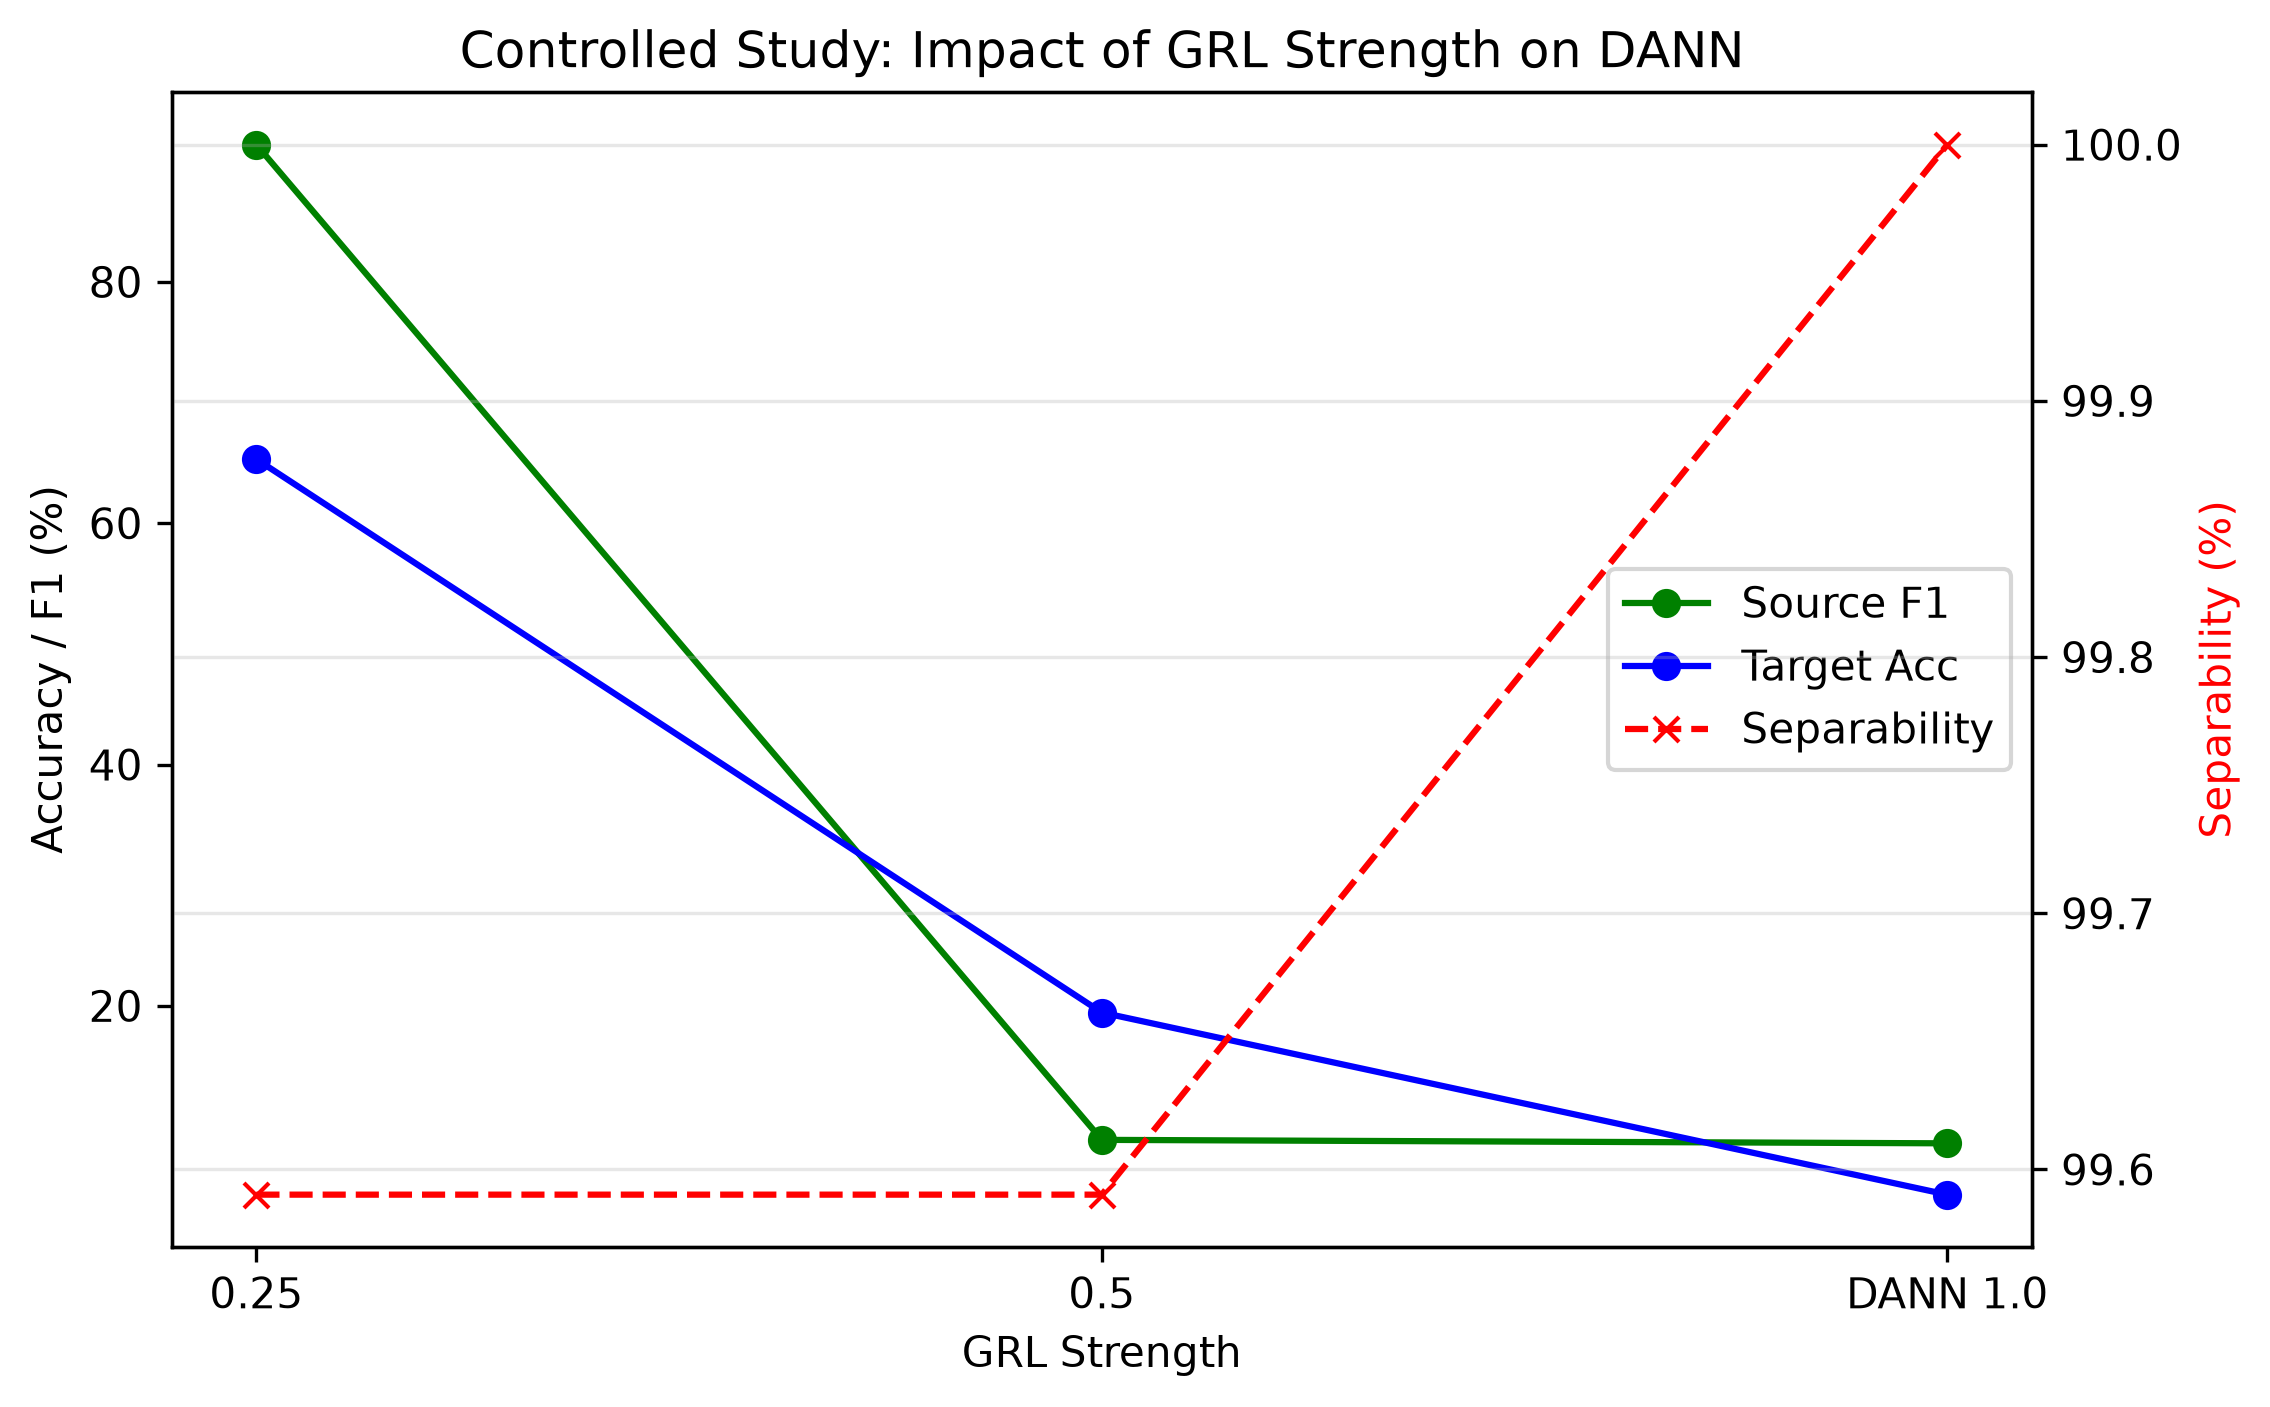
\includegraphics[scale=0.3]{../task2/results/controlled_study_plot.png}
  \caption{Impact of maximum Gradient Reversal Layer (GRL) strength on DANN source performance, target accuracy, and domain separability. The sharp drop in target accuracy at higher GRL strengths demonstrates the optimization trade-off where excessive alignment pressure causes feature collapse.}
  \label{fig:task2_controlled}
\end{figure}

\section{Domain Generalization}
\label{section:dg}


Domain generalization (DG) evaluates whether a model optimized on several observed source domains can successfully generalize to a novel, unseen environment. Unlike unsupervised domain adaptation, DG strictly prohibits any access to target-domain data during the training and validation phases. In this task, we investigate whether empirical risk minimization (ERM) across diverse source domains is sufficient for generalization, or if explicit interventions are required. We contrast ERM against two distinct generalization hypotheses: enforcing representation invariance by explicitly minimizing the discrepancy among the observed source domains, and encouraging local parameter stability by optimizing for flat loss landscapes. 

\subsection{Methodology}

\paragraph{Dataset and DG Protocol}
We continue our evaluation on the PACS dataset, utilizing Photo, Art Painting, and Cartoon as our labeled source domains. Crucially, following the rigorous evaluation protocol established by \citet{gulrajani2021in}, the Sketch domain is designated as a strictly unseen target environment; no Sketch images are exposed to the models during training, representation learning, checkpoint selection, or hyperparameter tuning.

\paragraph{Architecture and Optimization Baseline}
We maintain the exact architectural and optimization constraints established in the previous task: a pre-trained ResNet-18 backbone with a seven-class linear head. Each training batch contains exactly eight examples from each of the three source domains. To serve as our baseline, we directly reuse the Source-Only ERM checkpoint trained in Task 2, which optimizes the standard cross-entropy risk over the combined source domains without any explicit alignment penalties.

\paragraph{Generalization Strategies}
We evaluate two targeted interventions against the ERM baseline. DAN-DG adapts the Maximum Mean Discrepancy (MMD) mechanism from the standard UDA setting \citep{pmlr-v37-long15} to enforce marginal representation invariance strictly across the observed source domains. We apply the MMD penalty ($\lambda_{DG}=1$) to the 512-dimensional feature space, computing the average discrepancy over the three unordered pairs of source domains using the same multi-bandwidth RBF kernel configuration established in Task 2. Alternatively, SAM (Sharpness-Aware Minimization) \citep{foret2021sharpnessaware} seeks parameters residing in uniformly low-loss neighborhoods. Without explicitly penalizing domain discrepancies, SAM computes a normalized gradient-ascent perturbation (with a neighborhood radius $\rho=0.05$) and updates the model parameters using the cross-entropy loss evaluated at this perturbed, worst-case local point. An overview of the training process including optimization hyperparameters and the training and validation accuracy trajectories are provided in Appendix \ref{appendix:task3_training}.


\paragraph{Diagnostics and Controlled Study}
To quantify the residual domain-specific information encoded by the DG methods, we compute a source-domain separability score. We extract frozen representations from a balanced 70/30 split of the source validation sets and train a multinomial logistic regression classifier to predict the originating domain (Photo, Art Painting, or Cartoon), where chance performance is 33.3\%. To evaluate local parameter stability, we compute a standardized local sharpness proxy: the increase in cross-entropy loss after applying a single normalized gradient-ascent perturbation (radius 0.05) to a fixed validation batch. Finally, for our controlled design study, we systematically vary the neighborhood radius $\rho \in \{0.01, 0.05, 0.1\}$ in the SAM optimizer to directly investigate the trade-off between local flatness, source performance, and out-of-distribution generalization.

\subsection{Results and Analysis}

\paragraph{Source-Side Validation vs. Target Generalization}
Table~\ref{tab:task3_main} summarizes the generalization metrics across the three core strategies. Empirical risk minimization (ERM) yields high confidence during training, achieving a mean source F1 of 93.89\% and a worst-source performance (Art Painting) of 90.63\%. However, these aggregate source metrics are severely disconnected from out-of-distribution performance, as the model achieves only 57.52\% accuracy on the unseen Sketch domain. Furthermore, the strong source aggregates mask critical class-level vulnerabilities. As detailed in Table~\ref{tab:task3_per_class}, the ERM baseline fails entirely on classes like 'Horse' (39.2\%) and 'Elephant' (47.6\%) under the domain shift, demonstrating that models can perfectly minimize empirical risk on diverse source environments while still relying on superficial, domain-specific cues.

\paragraph{Representation Invariance and Discriminability Trade-offs}
DAN-DG explicitly addresses domain shift by minimizing the discrepancy among the observed source domains, successfully dropping the domain separability score from 88.16\% to 74.01\%. This resulting invariance significantly improves overall Sketch recognition, yielding a +13.34\% target accuracy gain over ERM. However, explicit feature alignment inadvertently destroys class-discriminative information for certain categories. While DAN-DG produces massive gains on 'Elephant' (+46.2\%) and 'Guitar' (+34.0\%), its accuracy on 'Dog' collapses by 46.0\% (Table~\ref{tab:task3_per_class}). By forcefully overlapping the marginal distributions of the source domains, the alignment penalty smeared the semantic boundaries between structurally similar animals, causing the network to misclassify dog input images as elephants and giraffes under the Sketch distribution.

\paragraph{Local Parameter Stability vs. Feature Alignment}
Sharpness-Aware Minimization (SAM) offers a distinctly different route to generalization. Rather than explicitly minimizing domain discrepancy, SAM searches for flat minima. As expected, SAM ($\rho=0.05$) drastically reduces the standardized local sharpness proxy ($\Delta \mathcal{L} = 0.1134$) compared to ERM (0.2996) and DAN-DG (0.3711). Despite being the "sharpest" model, DAN-DG achieves target accuracy (70.86\%) strictly comparable to the flattest model, SAM (70.63\%). This confirms that the ranking by local parameter stability does not strictly dictate the ranking by unseen domain generalization; domain invariance and local parameter flatness operate as distinct, independently viable mechanisms for robustness. Table~\ref{tab:task3_controlled} further illustrates that increasing SAM's perturbation radius monotonically improves domain separability and sharpness, but excessive regularization ($\rho=0.10$) disrupts the target accuracy trade-off.

\begin{table}[ht]
  \caption{Task 3 main evaluation metrics: Source performance, unseen target (Sketch) generalization, domain separability, and local sharpness. Both DAN-DG and SAM significantly outperform the ERM baseline on the unseen domain via distinct mechanisms.}
  \label{tab:task3_main}
  \centering
  \setlength{\tabcolsep}{4.5pt}
  \begin{tabular}{lccccc}
    \toprule
    Method & Mean Src (F1) & Worst Src (F1) & Tgt Acc (\%) & Sep. (\%) & Sharpness ($\Delta \mathcal{L}$) \\
    \midrule
    ERM & 93.89 & 90.63 & 57.52 & 88.16 & 0.2996 \\
    DAN-DG & 93.74 & 90.56 & 70.86 & 74.01 & 0.3711 \\
    SAM ($\rho=0.05$) & 94.76 & 91.12 & 70.63 & 86.51 & 0.1134 \\
    \bottomrule
  \end{tabular}
\end{table}

\begin{table}[ht]
  \caption{Controlled Study: Impact of perturbation radius ($\rho$) on SAM's generalization, domain separability, and local stability. Increasing the radius flattens the local loss landscape, but excessive perturbation yields diminishing returns on target accuracy.}
  \label{tab:task3_controlled}
  \centering
  \begin{tabular}{lcccc}
    \toprule
    Radius ($\rho$) & Tgt Acc (\%) & Tgt F1 (\%) & Sep. (\%) & Sharpness ($\Delta \mathcal{L}$) \\
    \midrule
    0.01 & 69.53 & 71.53 & 88.49 & 0.2228 \\
    0.05 (Base) & 70.63 & 72.07 & 86.51 & 0.1134 \\
    0.10 & 70.25 & 72.33 & 81.91 & 0.0819 \\
    \bottomrule
  \end{tabular}
\end{table}

\begin{table}[ht]
  \caption{Per-class target accuracy changes on Sketch relative to the ERM baseline. The severe degradation of the 'Dog' class under DAN-DG highlights how explicit source alignment can inadvertently destroy class-discriminative boundaries.}
  \label{tab:task3_per_class}
  \centering
  \begin{tabular}{lccc}
    \toprule
    Class & ERM Base (Acc) & DAN-DG ($\Delta$) & SAM 0.05 ($\Delta$) \\
    \midrule
    Dog & 0.817 & -0.460 & -0.377 \\
    Elephant & 0.476 & +0.462 & +0.426 \\
    Guitar & 0.503 & +0.340 & +0.350 \\
    Horse & 0.392 & +0.175 & +0.252 \\
    Person & 0.656 & -0.012 & +0.262 \\
    \bottomrule
  \end{tabular}
\end{table}

\section{Open-Set Recognition}
\label{section:osr}

Standard supervised classification relies heavily on the closed-set assumption: every test input is presumed to belong to a category observed during training. However, in real-world deployments, models frequently encounter novel inputs that fall entirely outside this known label space. Open-set recognition (OSR) augments standard classification by equipping the model with the capacity to identify and reject these unknown inputs rather than forcing a highly confident, erroneous prediction. In this section, we evaluate how different training objectives and scoring mechanisms handle this rejection task. We specifically distinguish between near-semantic unknowns—inputs that are visually or conceptually adjacent to known classes—and far-semantic unknowns, which lack substantial overlap with the training distribution. By comparing post-hoc novelty scoring against methods that explicitly alter the learned representation and decision boundaries, we investigate whether improving closed-set accuracy inherently solves open-set rejection.

\subsection{Methodology}

\paragraph{Datasets and Evaluation Protocol}
We designate the ten classes of the CIFAR-10 dataset as the known label space. To evaluate OSR capabilities, we construct a strict, evaluation-only dataset of unknown inputs sampled from 16 fixed CIFAR-100 classes. These unknowns are symmetrically divided into a near-semantic group (e.g., wolf, tractor, bus) and a far-semantic group (e.g., wardrobe, clock, mushroom) to isolate the impact of conceptual proximity on rejection performance. Rejection efficacy is quantified using the Area Under the Receiver Operating Characteristic curve (AUROC) and the False Positive Rate at 95\% True Positive Rate (FPR@95TPR). Crucially, the rejection threshold for the latter is calibrated exclusively using the known CIFAR-10 validation set to target a 95\% acceptance rate for in-distribution examples.

\paragraph{Architectures and Post-Hoc Baselines}
All experiments employ a CIFAR-appropriate ResNet-18 backbone, modified with a $3 \times 3$ stride-1 initial convolution and the removal of the initial max-pooling layer to process $32 \times 32$ spatial dimensions natively. We first train a Vanilla baseline utilizing standard cross-entropy and stochastic gradient descent. We extract its frozen logits and penultimate features to compare four post-hoc unknownness scores: normalized confidence via Maximum Softmax Probability (MSP) \citep{hendrycks2017a}, absolute logit magnitude via Maximum Logit Score (MLS), aggregate logit evidence via Energy-based scoring \citep{NEURIPS2020_f5496252}, and feature distance via the Mahalanobis metric. To test the hypothesis that stronger in-distribution generalization inherently aids rejection \citep{vaze2022opensetrecognitiongoodclosedset}, we train a second model, GCSC (Good Closed-Set Classifier), which injects heavy spatial and color distortions via random augmentation during training, subsequently evaluating its rejection capacity using MLS.

\paragraph{Placeholder and Reciprocal Learning}
We contrast these post-hoc techniques with proactive OSR frameworks that explicitly restructure the latent space. PROSER \citep{Zhou_2021_CVPR} prepares the network for novel inputs by jointly learning dummy classifier placeholders and synthetic data placeholders. Because genuine unknown examples are strictly withheld, we generate data placeholders via manifold mixup, blending representations from distinct known classes to simulate unknown-like boundary regions. These proxy representations are actively pushed toward the dummy classifiers to tighten the known-class decision boundaries. Finally, we implement Reciprocal Point Learning (RPL) \citep{Chen2020}, which shifts the classification paradigm from bounding what a class is to learning what it is not. RPL introduces an open-space regularization term and learns a reciprocal point for each known category. By pushing known-class features away from their corresponding reciprocal points, the network naturally bounds the known latent space, allowing us to reject test inputs that fall insufficiently far from these reciprocal anchors.

An overview of the training process including optimization hyperparameters and the training and validation accuracy trajectories are provided in Appendix \ref{appendix:task4_training}.

\subsection{Results and Analysis}

\paragraph{Post-Hoc Novelty Scoring and Metric Sensitivities}
Table~\ref{tab:osr_posthoc} evaluates the capacity of different post-hoc scoring mechanisms to reject unknown inputs using the frozen Vanilla baseline. Maximum Softmax Probability (MSP) exhibits the weakest overall performance, accepting 71.88\% of near unknowns and 60.25\% of far unknowns at a 95\% true positive rate. This failure occurs because the softmax function normalizes logits into a probability distribution, artificially inflating confidence even when all raw logit magnitudes are uniformly low. By bypassing the softmax bottleneck, Maximum Logit Score (MLS) and Energy scoring preserve the absolute, unnormalized distance to the decision boundary, yielding nearly identical and vastly superior rejection rates (e.g., dropping near-unknown FPR to $\sim$68\%). The Mahalanobis distance strictly captures the Gaussian cluster geometry of the learned representations, making it highly effective for identifying structurally distant far unknowns (achieving the highest Far AUROC of 0.9145). However, it struggles more than MLS on near unknowns, as semantically adjacent concepts often map to the periphery of the known-class feature clusters.

\paragraph{Semantic Proximity and Failure Analysis}
The stark discrepancy between near and far OSR metrics across all methods underscores how semantic similarity dictates rejection difficulty. Figure~\ref{fig:osr_distributions} demonstrates that near unknowns heavily overlap with the known-class score distributions, whereas far unknowns form a slightly more distinct, separable mass. An inspection of specific failures passing the validated MLS threshold ($\tau = -5.8116$) reveals the underlying mechanics of this overlap. Near-unknown failures are highly semantically plausible: the network confidently absorbs visually adjacent concepts into its known categories, predicting a 'wolf' as a 'dog' (MLS: -8.3052), a 'leopard' as a 'cat' (MLS: -7.3185), and a 'pickup truck' as a 'truck' (MLS: -9.9977). Conversely, far-unknown failures expose the model's reliance on superficial low-level features when semantic overlap is absent. The network inappropriately accepts a 'chair' as an 'airplane' (MLS: -7.4270), a 'bottle' as a 'bird' (MLS: -7.8000), and a 'bowl' as a 'truck' (MLS: -9.1805), indicating that local texture or edge responses can occasionally trigger high logit activations even for completely unrelated geometries.

\paragraph{The Impact of Augmentation on Decision Boundaries}
Table~\ref{tab:osr_interventions} demonstrates that the heavy spatial and color distortions introduced in the GCSC model simultaneously improve closed-set accuracy (94.67\% to 95.15\%) and open-set recognition. By forcing the network to maintain classification under aggressive transformations, RandAugment tightens the decision boundaries around the known classes. This leads to a substantial improvement in far-unknown rejection, dropping the Far FPR from 48.88\% (Vanilla) to 41.63\% (GCSC). However, this boundary tightening provides diminishing returns for near unknowns (Near FPR drops only to 63.38\%); augmentation makes the known classes more robust, but it cannot structurally separate concepts that inherently share semantic sub-features (e.g., a wolf and a dog).

\paragraph{Proactive OSR: Placeholders and Reciprocal Points}
PROSER and RPL attempt to proactively restructure the latent space during training, with highly divergent results. PROSER successfully maintains closed-set accuracy (94.61\%) while introducing dummy classifiers and data placeholders. However, its efficacy relies heavily on its custom placeholder-based detection score. Using MLS, PROSER actually degrades OSR performance relative to the baseline. Using its custom score, PROSER achieves an exceptional Far AUROC (0.9173) and Far FPR (44.25\%), but completely fails on near unknowns (Near FPR: 74.50\%). This exposes a critical limitation of manifold mixup: interpolating between two known classes (e.g., mixing 'cat' and 'car') generates artificial boundaries that help reject arbitrary out-of-distribution noise, but these synthetic proxy-unknowns do not accurately simulate the specific feature vectors of semantically adjacent unknowns like 'wolf'. Finally, Reciprocal Point Learning (RPL) suffers massive degradation across all metrics, dropping to 93.75\% CSA and a catastrophic Near AUROC of 0.6340. Forcing a ResNet-18 to map all known classes away from specific reciprocal anchors while simultaneously regularizing the open space proves exceptionally difficult to optimize within the epoch budget, heavily distorting the underlying representations.

\begin{table}[ht]
  \caption{Vanilla model post-hoc novelty scores. Unnormalized logit magnitudes (MLS, Energy) and feature distances (Mahalanobis) significantly outperform normalized confidence (MSP) across all rejection thresholds.}
  \label{tab:osr_posthoc}
  \centering
  \begin{tabular}{lccccc}
    \toprule
    Score & Near AUROC & Far AUROC & All AUROC & FPR (Near) & FPR (Far) \\
    \midrule
    MSP & 0.8108 & 0.8939 & 0.8524 & 0.7188 & 0.6025 \\
    MLS & 0.7911 & 0.8875 & 0.8393 & 0.6775 & 0.4888 \\
    Energy & 0.7907 & 0.8881 & 0.8394 & 0.6825 & 0.4938 \\
    Mahalanobis & 0.7966 & 0.9145 & 0.8555 & 0.7125 & 0.5050 \\
    \bottomrule
  \end{tabular}
\end{table}

\begin{table}[ht]
  \caption{Model interventions comparing closed-set accuracy (CSA) and OSR performance. Strong data augmentation (GCSC) uniformly improves both recognition and rejection, whereas proactive architectures present severe trade-offs.}
  \label{tab:osr_interventions}
  \centering
  \begin{tabular}{lcccccc}
    \toprule
    Model & Score & CSA (\%) & Near AUC & Far AUC & FPR (Near) & FPR (Far) \\
    \midrule
    VANILLA & MLS & 94.67 & 0.7911 & 0.8875 & 0.6775 & 0.4888 \\
    GCSC & MLS & 95.15 & 0.8145 & 0.9121 & 0.6338 & 0.4163 \\
    PROSER & MLS & 94.61 & 0.7620 & 0.8792 & 0.7225 & 0.5075 \\
    PROSER & Custom & - & 0.7527 & 0.9173 & 0.7450 & 0.4425 \\
    RPL & Custom & 93.75 & 0.6340 & 0.7631 & 0.7412 & 0.5625 \\
    \bottomrule
  \end{tabular}
\end{table}

\begin{figure}[ht]
  \centering
  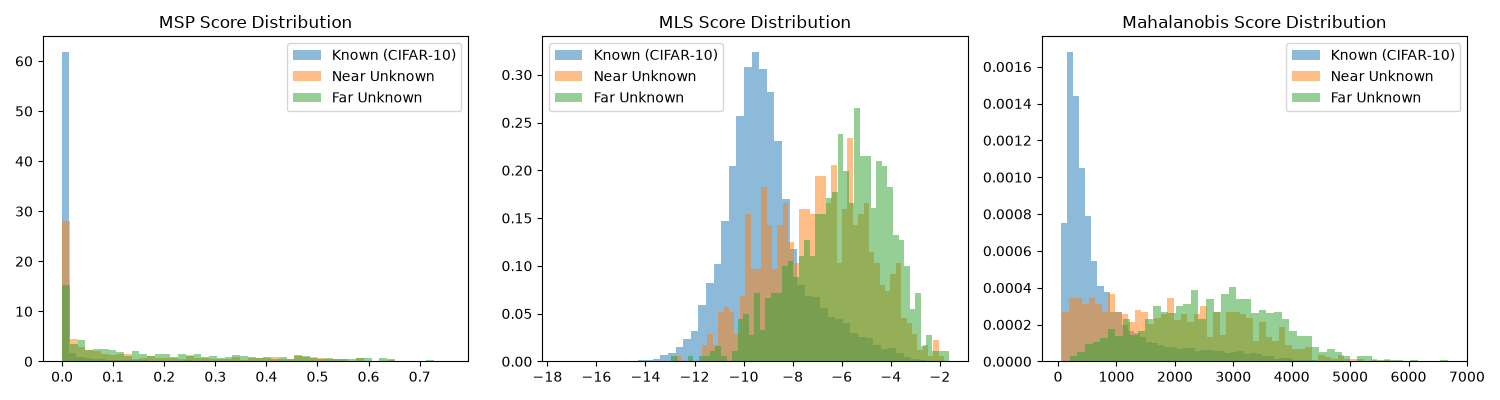
\includegraphics[width=\textwidth]{../task4/results/score_distributions.png}
  \caption{Score distributions for known and unknown classes across three post-hoc mechanisms. The substantial overlap of the orange near-unknown distributions highlights the inherent difficulty of rejecting semantically adjacent inputs.}
  \label{fig:osr_distributions}
\end{figure}

\section{Cross-Task Discussion}

\paragraph{Visual Cues and Distribution Shift}
In Section \ref{section:biases}, controlled interventions revealed that standard ImageNet-trained convolutional networks are relatively more texture-bias, whereas self-attention mechanisms and contrastive pretraining prioritize global shape. This architectural vulnerability explains the failure patterns observed under the PACS domain shifts in Sections \ref{section:uda} and \ref{section:dg}. The transition from the Photo domain to the Sketch domain inherently strips away chromatic information and local texture, leaving only raw geometric edges. Consequently, the empirical risk minimization (ERM) baseline struggled significantly, as it over-relied on domain-specific textures and contextual backgrounds that were absent in the Sketch environment.

\paragraph{Invariance versus Discriminability}
A central premise of UDA is that reducing the statistical distinguishability of domains improves generalization transfer. Across Sections \ref{section:uda} and \ref{section:dg}, our results demonstrate this assumption is overly simplistic. Marginal alignment successfully minimized domain separability but induced catastrophic negative transfer, effectively destroying target recognition. By forcing global distribution matching without regard for class structure, the alignment penalties smeared semantically distinct categories together into a collapsed feature space. Even when pairwise source alignment improved aggregate unseen domain accuracy, it simultaneously caused severe class-specific accuracy collapse. This confirms that enforcing representation invariance indiscriminately removes critical class-discriminative boundaries alongside domain-specific noise.

\paragraph{The Importance of Target Domain Access}
The stark performance contrast between target-aware DAN in Section \ref{section:uda} (2.04\% Sketch accuracy) and target-free DAN-DG in Section \ref{section:dg} (70.86\% Sketch accuracy) highlights the risks of prematurely utilizing unlabeled target data. Attempting to explicitly align the highly divergent marginal distributions of photorealistic sources against raw edge-map sketches forced the network to discard essential semantic features. Conversely, aligning the structurally compatible observed source domains produced a generalized representation that transferred highly effectively without ever observing the target. However, a strict causal attribution is limited, as the former aligned a pooled source distribution against the target, while the latter computed pairwise discrepancies strictly between individual source environments.

\paragraph{Recognition versus Rejection}
Section \ref{section:osr} demonstrated that representations optimized strictly for closed-set accuracy are not inherently equipped to handle semantic novelty. While heavy augmentation improved both closed-set accuracy and the rejection of structurally distant far-unknowns, it provided minimal benefit for near-semantic unknowns. PROSER attempted to proactively tighten decision boundaries using proxy data placeholders generated via manifold mixup. However, synthetic interpolations between distinct known classes failed to accurately simulate the feature geometries of semantically adjacent anomalies. This confirms that improving a classifier's ability to confidently recognize known classes does not automatically impart the compact structural boundaries required to safely reject near-semantic anomalies.

\section{Conclusion}

This study systematically explored the limitations of the independent and identically distributed (IID) assumption through the lenses of inductive biases, domain adaptation, domain generalization, and open-set recognition. Our findings synthesize into a unified principle for robust representation learning: a reliable model must preserve global structural semantics (shape) over local textures to survive natural distribution shifts. It should suppress domain-specific stylistic variations, but it must do so conditionally; enforcing naive statistical invariance ultimately destroys the discriminability of the latent space. Finally, rather than forcing every input into a known category via normalized probabilities, robust models must leverage unnormalized distance metrics to reject anomalous inputs that fall outside the established, bounded semantic manifold. By jointly addressing what to preserve, what to suppress, and when to reject, we can bridge the gap between controlled empirical risk minimization and unpredictable real-world deployment.

\newpage

{
\small
\bibliographystyle{unsrtnat}
\bibliography{refs} 
}

\newpage

\appendix

\section{Training Loss Curves and Validation Accuracy Trajectories}

\subsection{Linear Classifier Training on a CNN, ViT, and CLIP Backbone}
\label{appendix:task1_training}

To evaluate the learned representations, we follow a standard linear probing protocol. The weights of all pre-trained backbones are kept strictly frozen, and we train a single linear classifier head on top of the extracted features for each model. 

To tune the linear heads and prevent overfitting, we take the official training partition of the dataset and perform a stratified 80/20 training/validation split, ensuring class distributions remain balanced. A fixed random seed of 6304 is used for this split.

Each linear classifier is trained for a maximum of 50 epochs. We monitor validation accuracy at the end of each epoch and apply early stopping with a patience of five epochs. To ensure a fair comparison across all backbones, the initialization of the classifier heads and the training loop are both governed by the same random seed (6304). The complete list of hyperparameters is detailed in Table \ref{tab:linear_hyperparams}. The training and validation accuracy trajectories can be seen in Figure \ref{fig:task1_training}.

\begin{table}[h]
\centering
\caption{Hyperparameter values used for the linear classifier head training. These hyperparameters were kept constant while training the linear heads of all 3 architectures.}
\label{tab:linear_hyperparams}
\begin{tabular}{ll}
\toprule
\textbf{Hyperparameter} & \textbf{Value} \\
\midrule
Optimizer & AdamW \\
Learning Rate & $10^{-3}$ \\
Weight Decay & $10^{-4}$ \\
Max Epochs & 50 \\
Early Stopping Patience & 5 epochs (on val. accuracy) \\
Random Seed & 6304 \\
\bottomrule
\end{tabular}
\end{table}

\begin{figure}[ht]
    \centering
    % First subfigure
    \begin{subfigure}{0.45\textwidth}
        \centering
        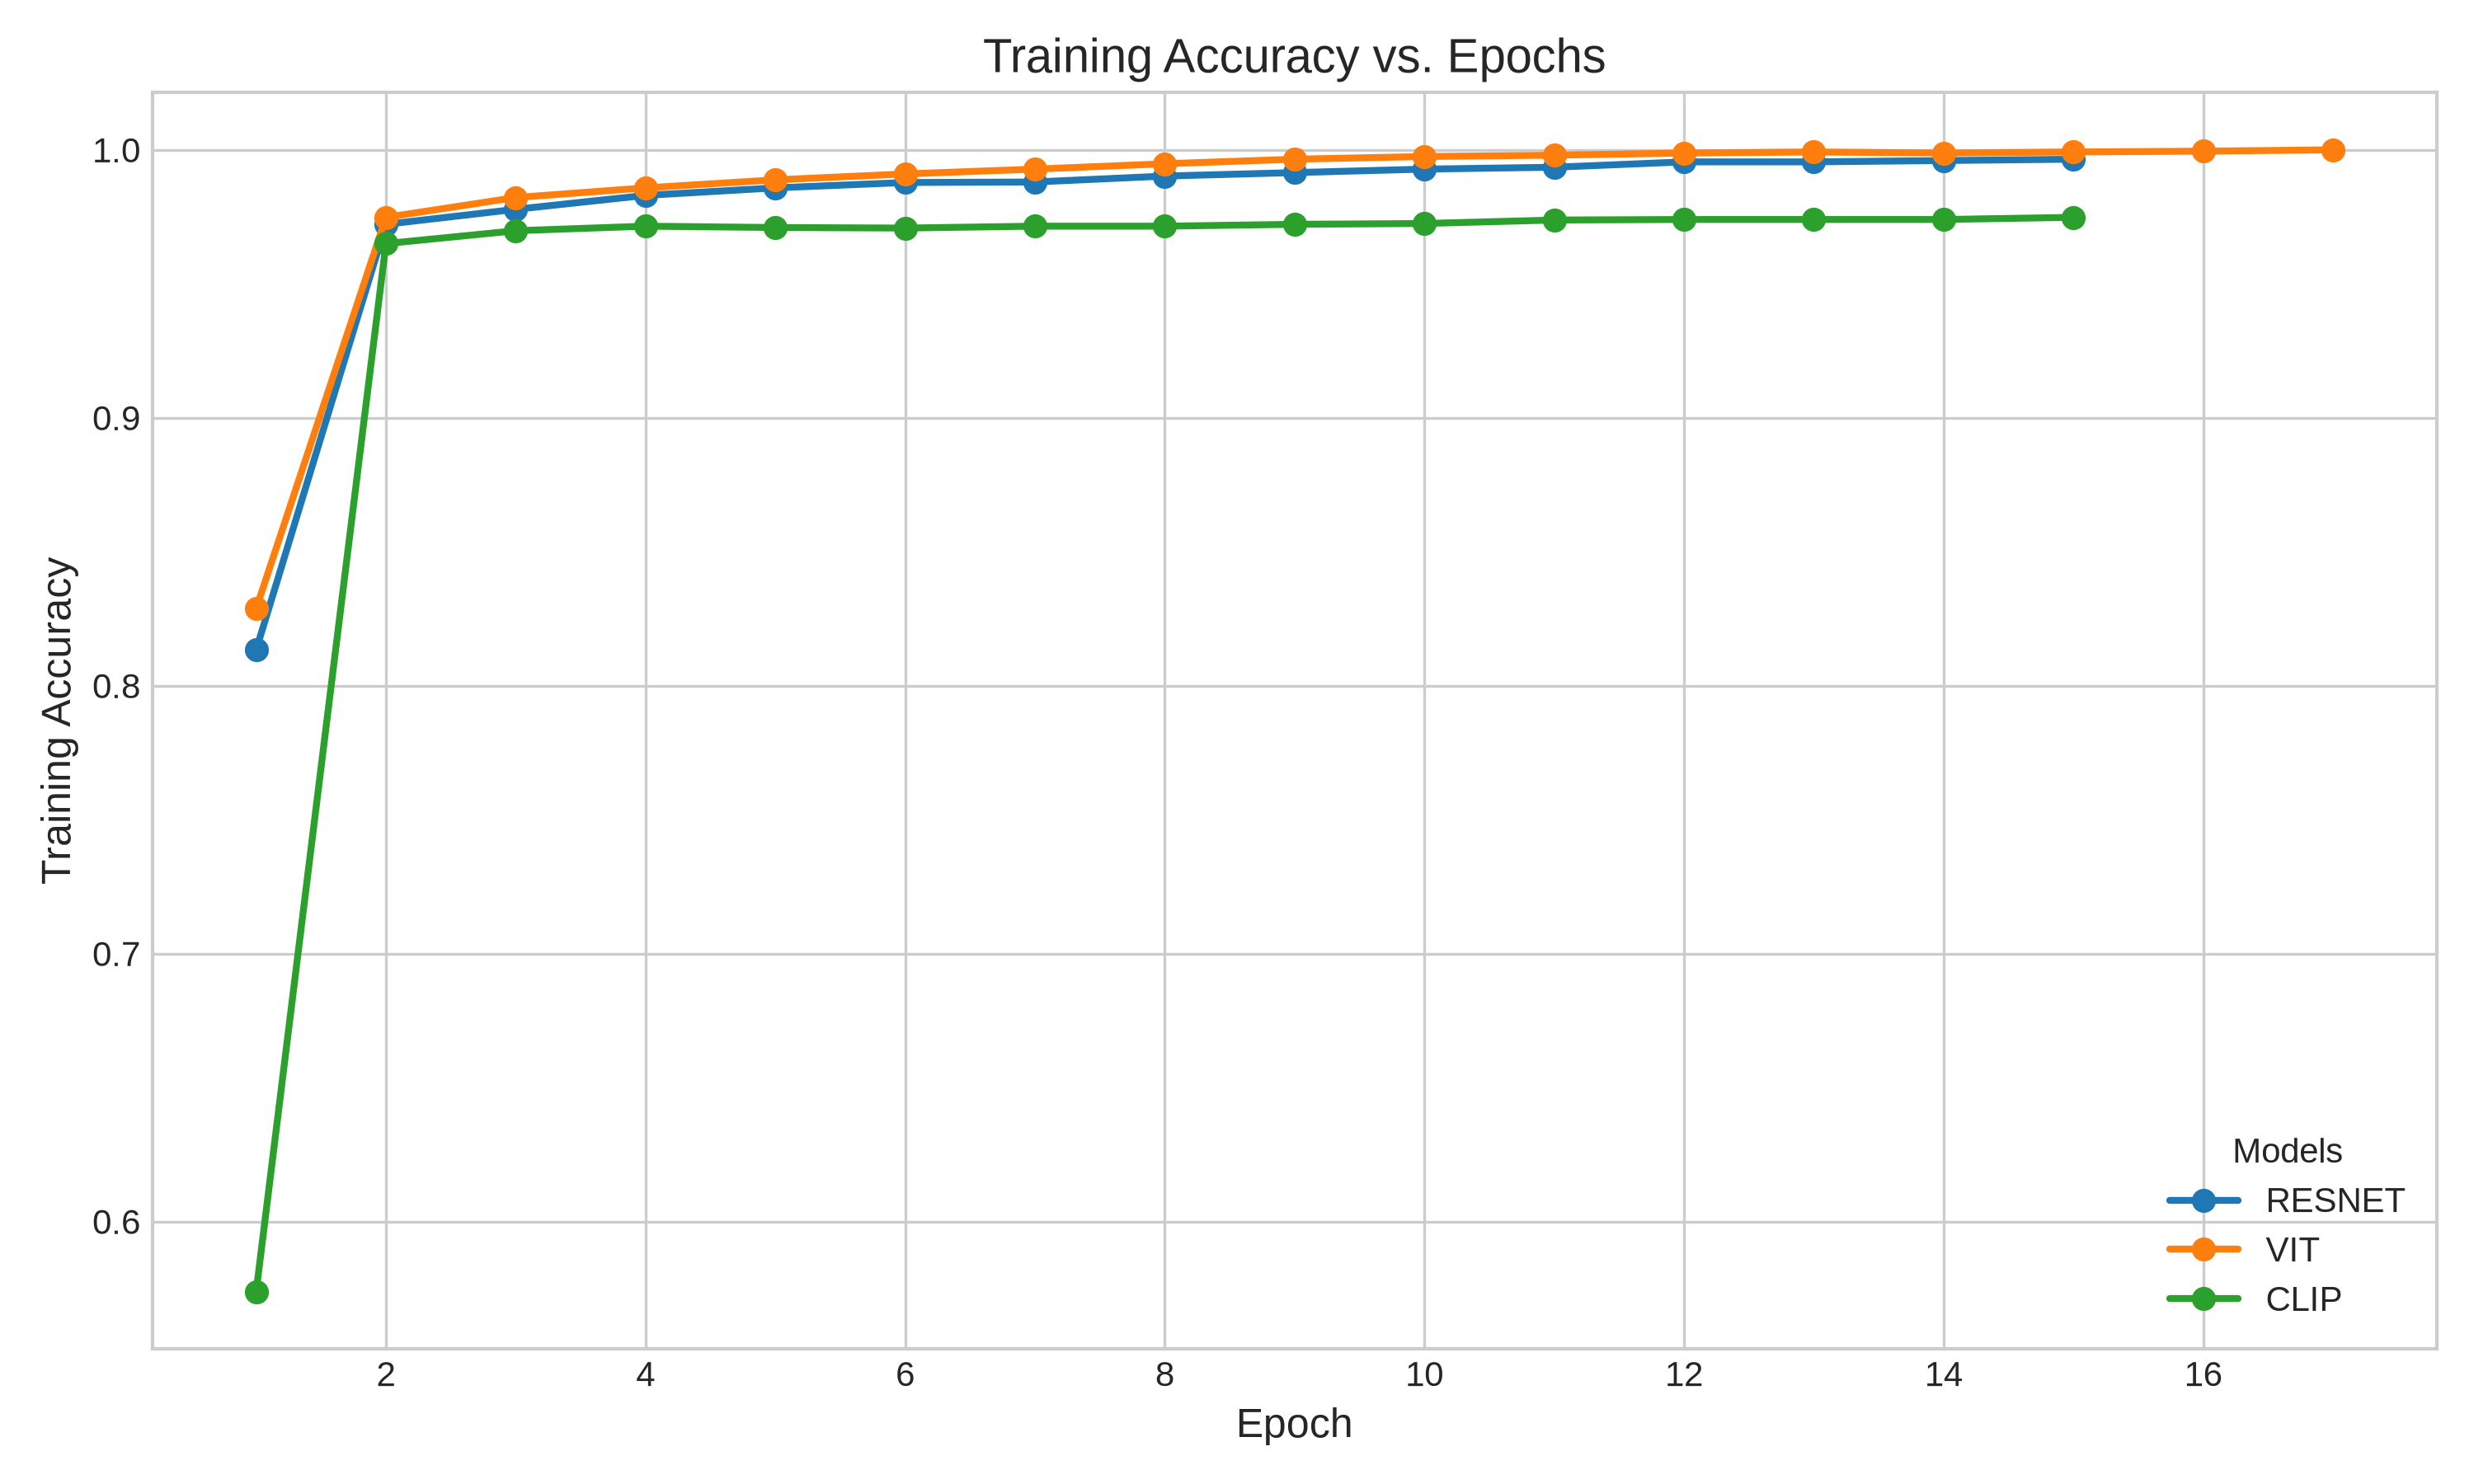
\includegraphics[width=\textwidth]{../task1/results/training_loss.png}
        \caption{Training Accuracy}
    \end{subfigure}
    \hfill
    % Second subfigure
    \begin{subfigure}{0.45\textwidth}
        \centering
        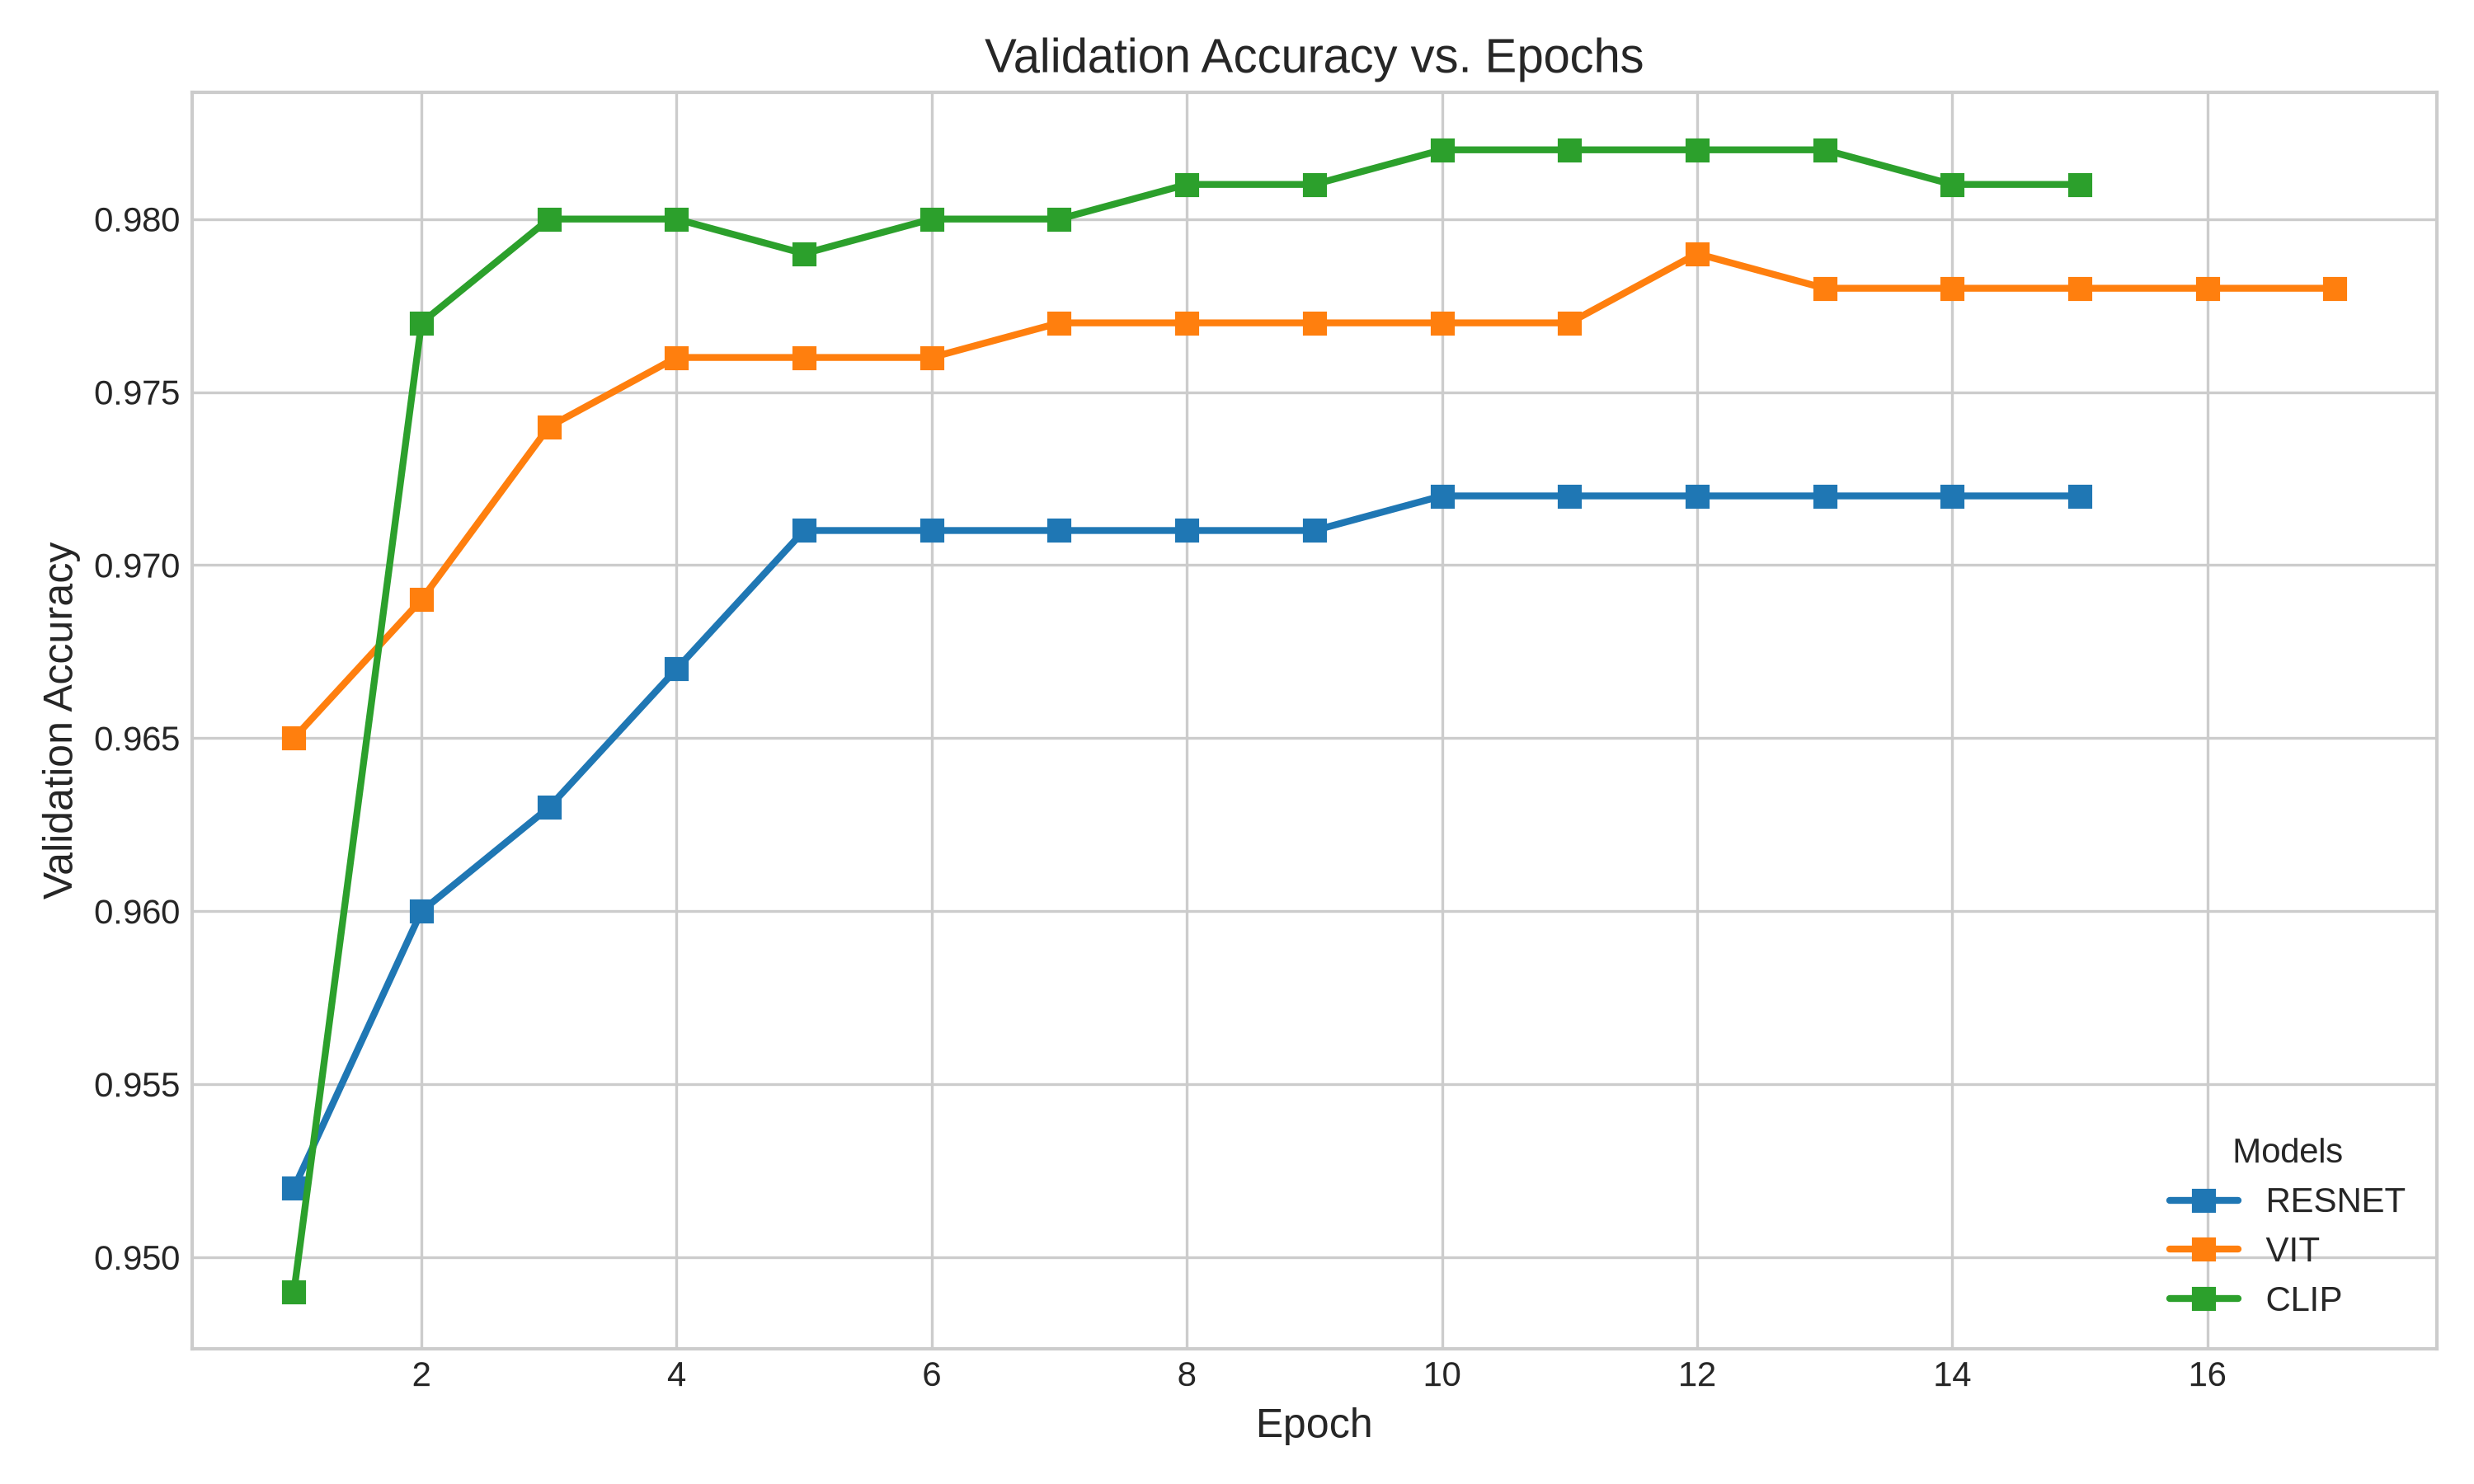
\includegraphics[width=\textwidth]{../task1/results/validation_acc.png}
        \caption{Validation Accuracy}
    \end{subfigure}
    
    \caption{Graphs plotting the training and validation accuracies of ResNet, ViT, and CLIP architectures with a linear classifier head. The effects of early stopping here is also visible as no epochs are recorded past the 18th epoch.}
    \label{fig:task1_training} 
\end{figure}

\subsection{UDA Training Trajectories and Optimization Diagnostics}
\label{appendix:task2_training}

To evaluate the unsupervised domain adaptation paradigms, all models were trained using a pre-trained ResNet-18 backbone and a randomly initialized linear classification head. Input images were resized to $256 \times 256$ and augmented with $224 \times 224$ random crops and horizontal flipping during training. To prevent implicit adaptation to the source-target batch mixture, all Batch Normalization running statistics were strictly frozen at their pre-trained ImageNet values. Training utilized the AdamW optimizer with a learning rate of $10^{-4}$ and weight decay of $10^{-4}$ for a maximum of 30 epochs. Each training batch was perfectly balanced, containing 24 source examples (eight from Photo, Art Painting, and Cartoon, respectively) and 24 unlabeled Sketch target examples. To prevent overfitting, early stopping was enforced if the mean source-validation macro-F1 score did not improve for five consecutive epochs. The baseline alignment strengths were set to $\lambda_{MMD}=1$ for DAN, and a standard progressive gradient-reversal schedule $\alpha(p)$ peaking at a unit weight for both DANN and CDAN (prior to our controlled study, which varied the maximum gradient-reversal strength in DANN). 

\begin{figure}[ht]
  \centering
  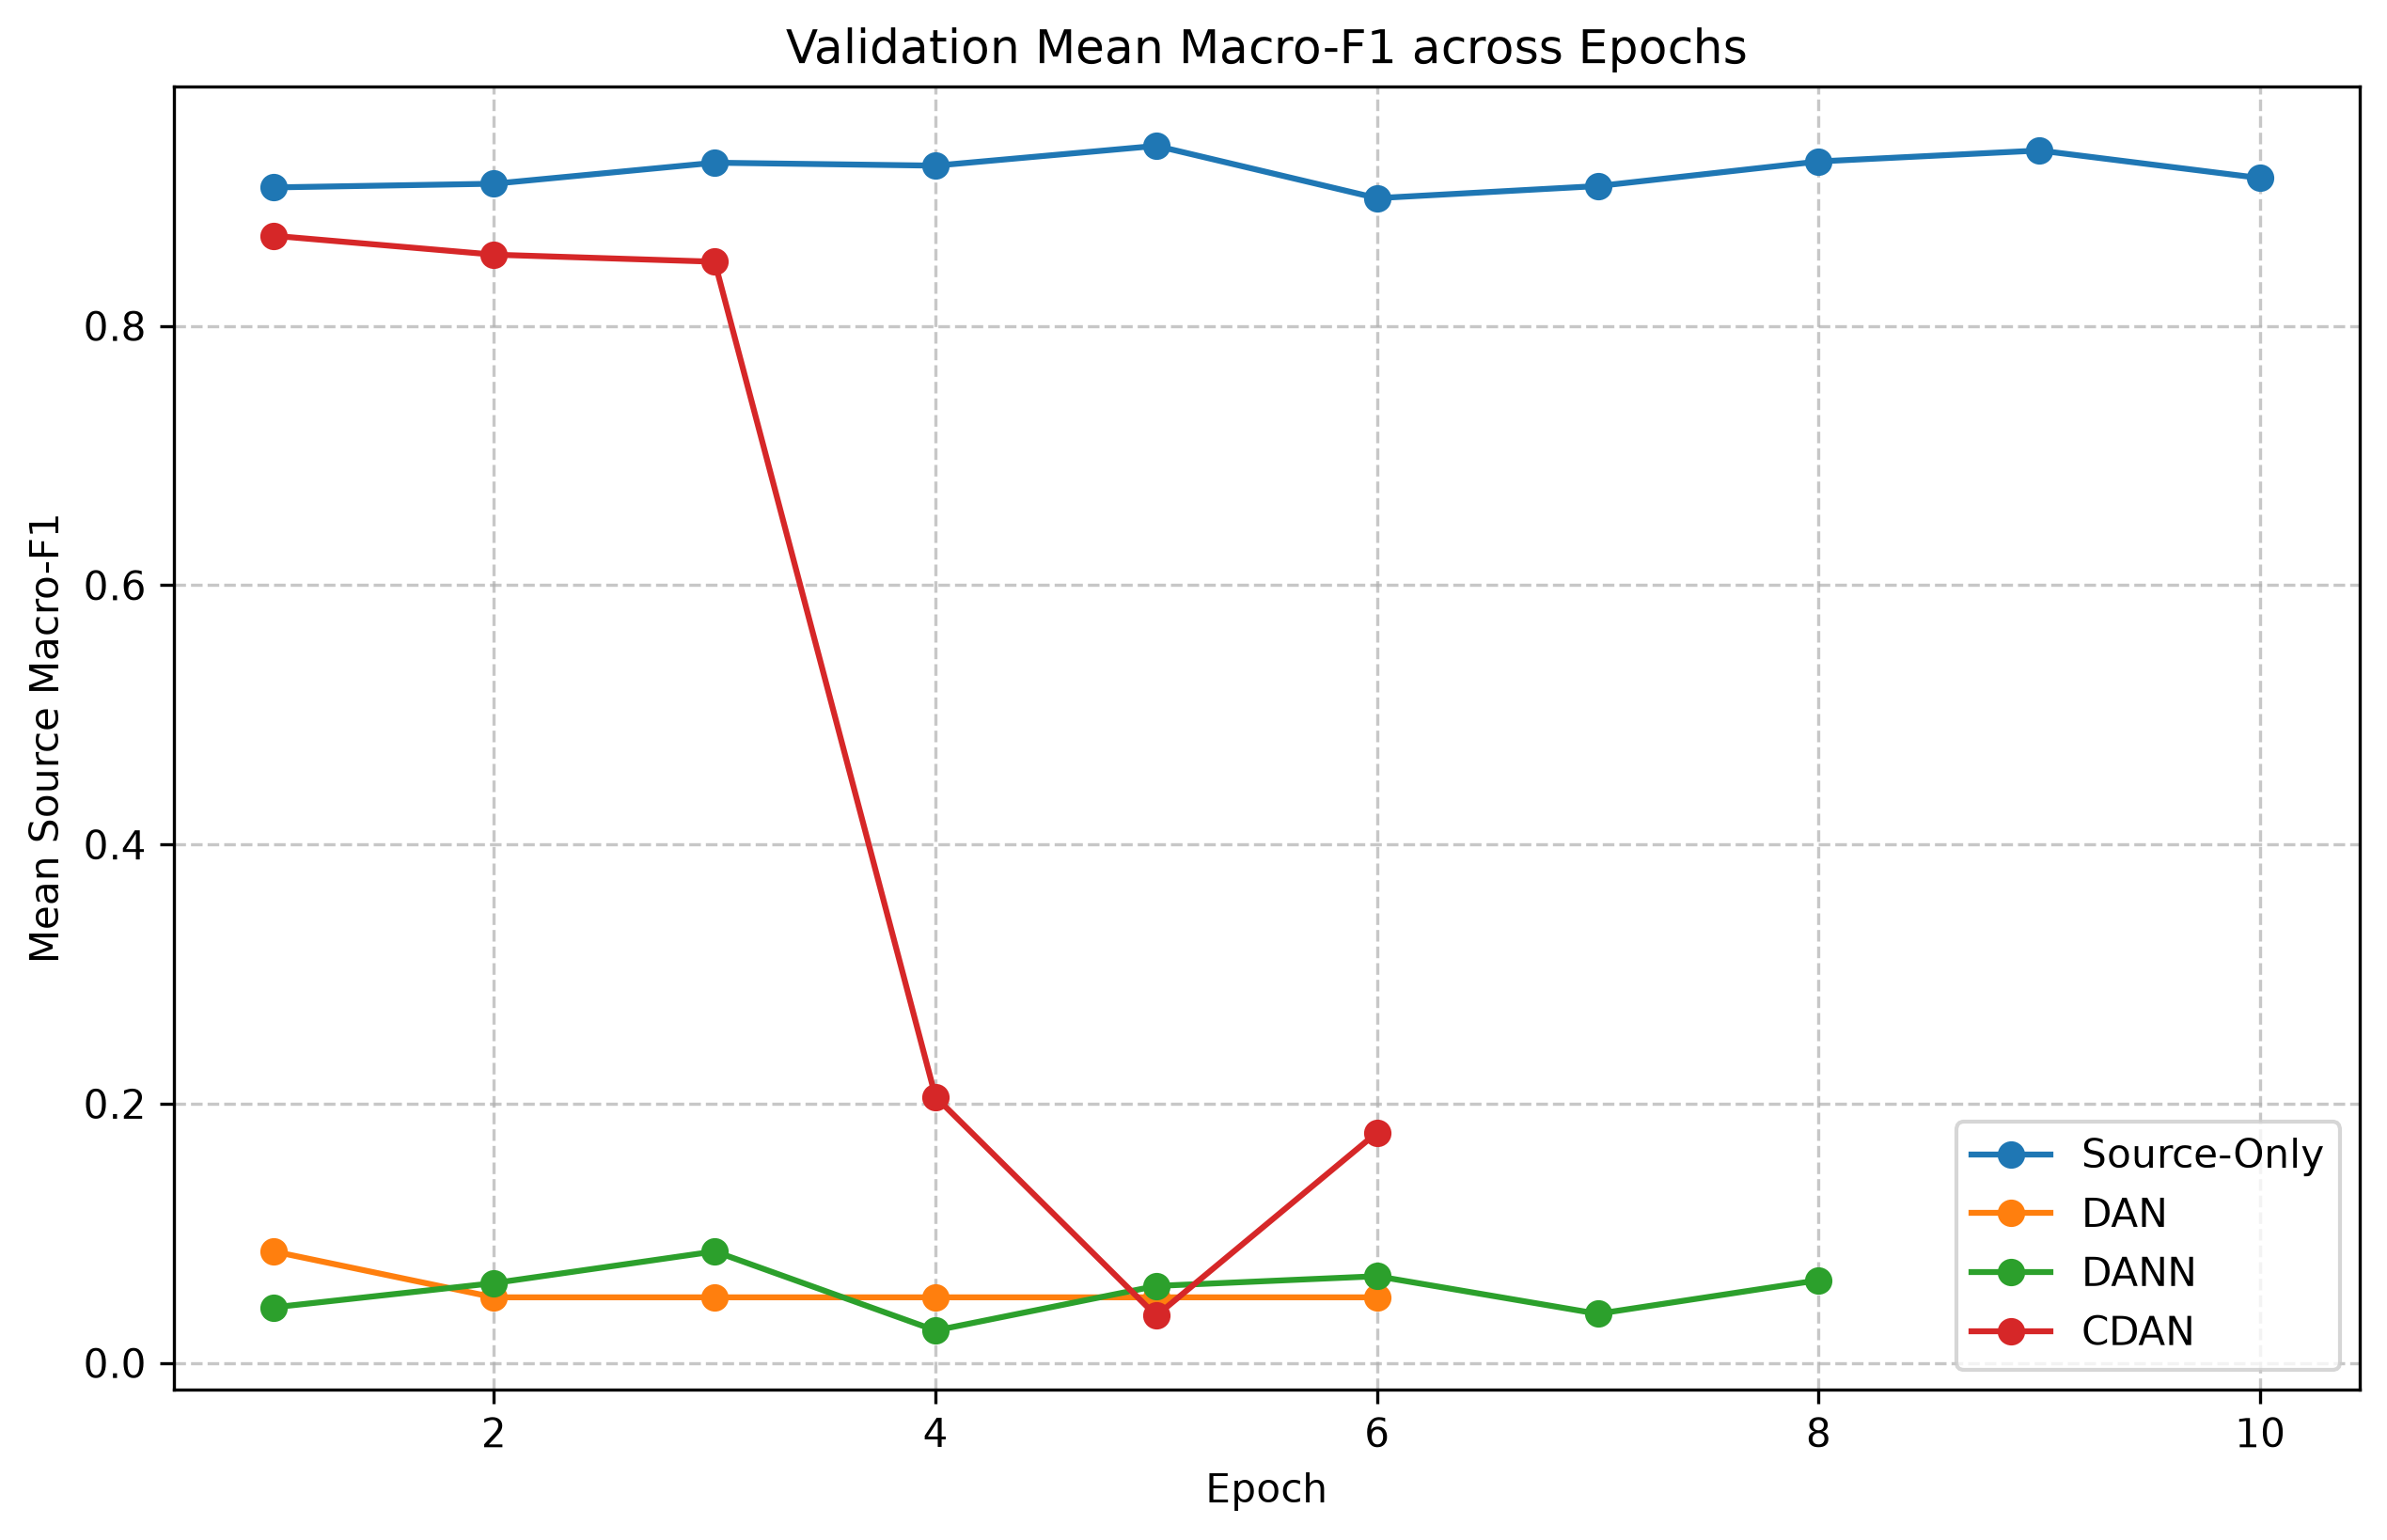
\includegraphics[width=0.8\textwidth]{../task2/results/training_curves.png}
  \caption{Validation Mean Source Macro-F1 across training epochs for the four UDA paradigms. The rapid termination of all adaptation methods highlights severe optimization instability and feature collapse under baseline alignment hyperparameters.}
  \label{fig:task2_training_curves}
\end{figure}

Figure~\ref{fig:task2_training_curves} illustrates the training trajectories for the four paradigms. Notably, no model training survived past epoch 10. This early termination is a direct consequence of the early stopping criterion; because the adaptation methods either failed to converge or rapidly degraded, the validation macro-F1 failed to improve over the 5-epoch patience window, halting the training well before the 30-epoch budget.

The training curves reveal severe optimization instabilities inherent to the architectural differences of each paradigm. The Source-Only model exhibits stable, high performance ($\approx0.9$ macro-F1) because it optimizes a standard cross-entropy objective without any adversarial or discrepancy penalties. Conversely, DAN and DANN exhibit a catastrophic failure to learn from initialization, with macro-F1 scores stagnating below 0.1. For DAN, the immediate application of the MMD penalty ($\lambda_{MMD}=1$) likely overwhelms the classification loss. It forces the marginal distributions of the unadapted features to match before the randomly initialized classifier head can establish meaningful decision boundaries, destroying class discriminability. Similarly, in DANN, despite the progressive gradient-reversal schedule, the domain discriminator rapidly overpowers the feature extractor. The combination of frozen Batch Normalization statistics and strong, early alignment gradients likely pushes the latent representations into a collapsed space where ImageNet statistics are no longer valid, rendering the features useless for classification.

CDAN exhibits a uniquely delayed collapse. Because CDAN conditions the domain discriminator on the outer product of the feature vector and the classifier's probability vector ($f \otimes p$), the initial domain penalty remains weak while the classifier's predictions ($p$) are uniform and uncertain. This allows the model to learn the source task effectively for the first three epochs, reaching an F1 score comparable to the Source-Only baseline. However, once the classifier becomes confident, the structured signal fed to the conditional discriminator strengthens dramatically. The resulting aggressive gradient reversal forces the generator to fool the discriminator by collapsing the probability vectors or disrupting the feature space entirely, causing the precipitous drop in accuracy observed after epoch 3.

\subsection{Domain Generalization Training Trajectories and Optimization Diagnostics}
\label{appendix:task3_training}

To rigorously evaluate the domain generalization paradigms, we strictly adhered to a target-free protocol. In contrast to unsupervised domain adaptation, the Sketch target domain was completely withheld during all phases of training, representation learning, checkpoint selection, and hyperparameter tuning. Checkpoints for all generalization models were selected solely based on the highest mean macro-F1 score across the three source validation domains (Photo, Art Painting, and Cartoon).

All models were initialized with a pre-trained ResNet-18 backbone and a randomly initialized seven-class linear classification head. Optimization was performed using AdamW with a learning rate of $10^{-4}$ and a weight decay of $10^{-4}$, capped at a maximum budget of 30 epochs. To prevent implicit domain adaptation via batch statistics, all Batch Normalization running means and variances were strictly frozen at their pre-trained ImageNet values. Training utilized perfectly balanced batches comprising eight examples from each of the three observed source domains.

We evaluated three distinct training objectives. The Empirical Risk Minimization (ERM) baseline—directly transferred from the unadapted Source-Only model in our prior adaptation experiments—optimizes standard cross-entropy across the pooled source domains. DAN-DG applies a pairwise Maximum Mean Discrepancy (MMD) penalty to every combination of the observed source domains to enforce source-invariance, utilizing the same multi-bandwidth RBF kernel configuration established previously. Finally, Sharpness-Aware Minimization (SAM) explores the local parameter space by computing a normalized gradient-ascent perturbation (with a baseline radius of $\rho=0.05$) before executing the optimization step, enforcing local loss flatness without explicitly penalizing domain discrepancies.

\begin{figure}[ht]
  \centering
  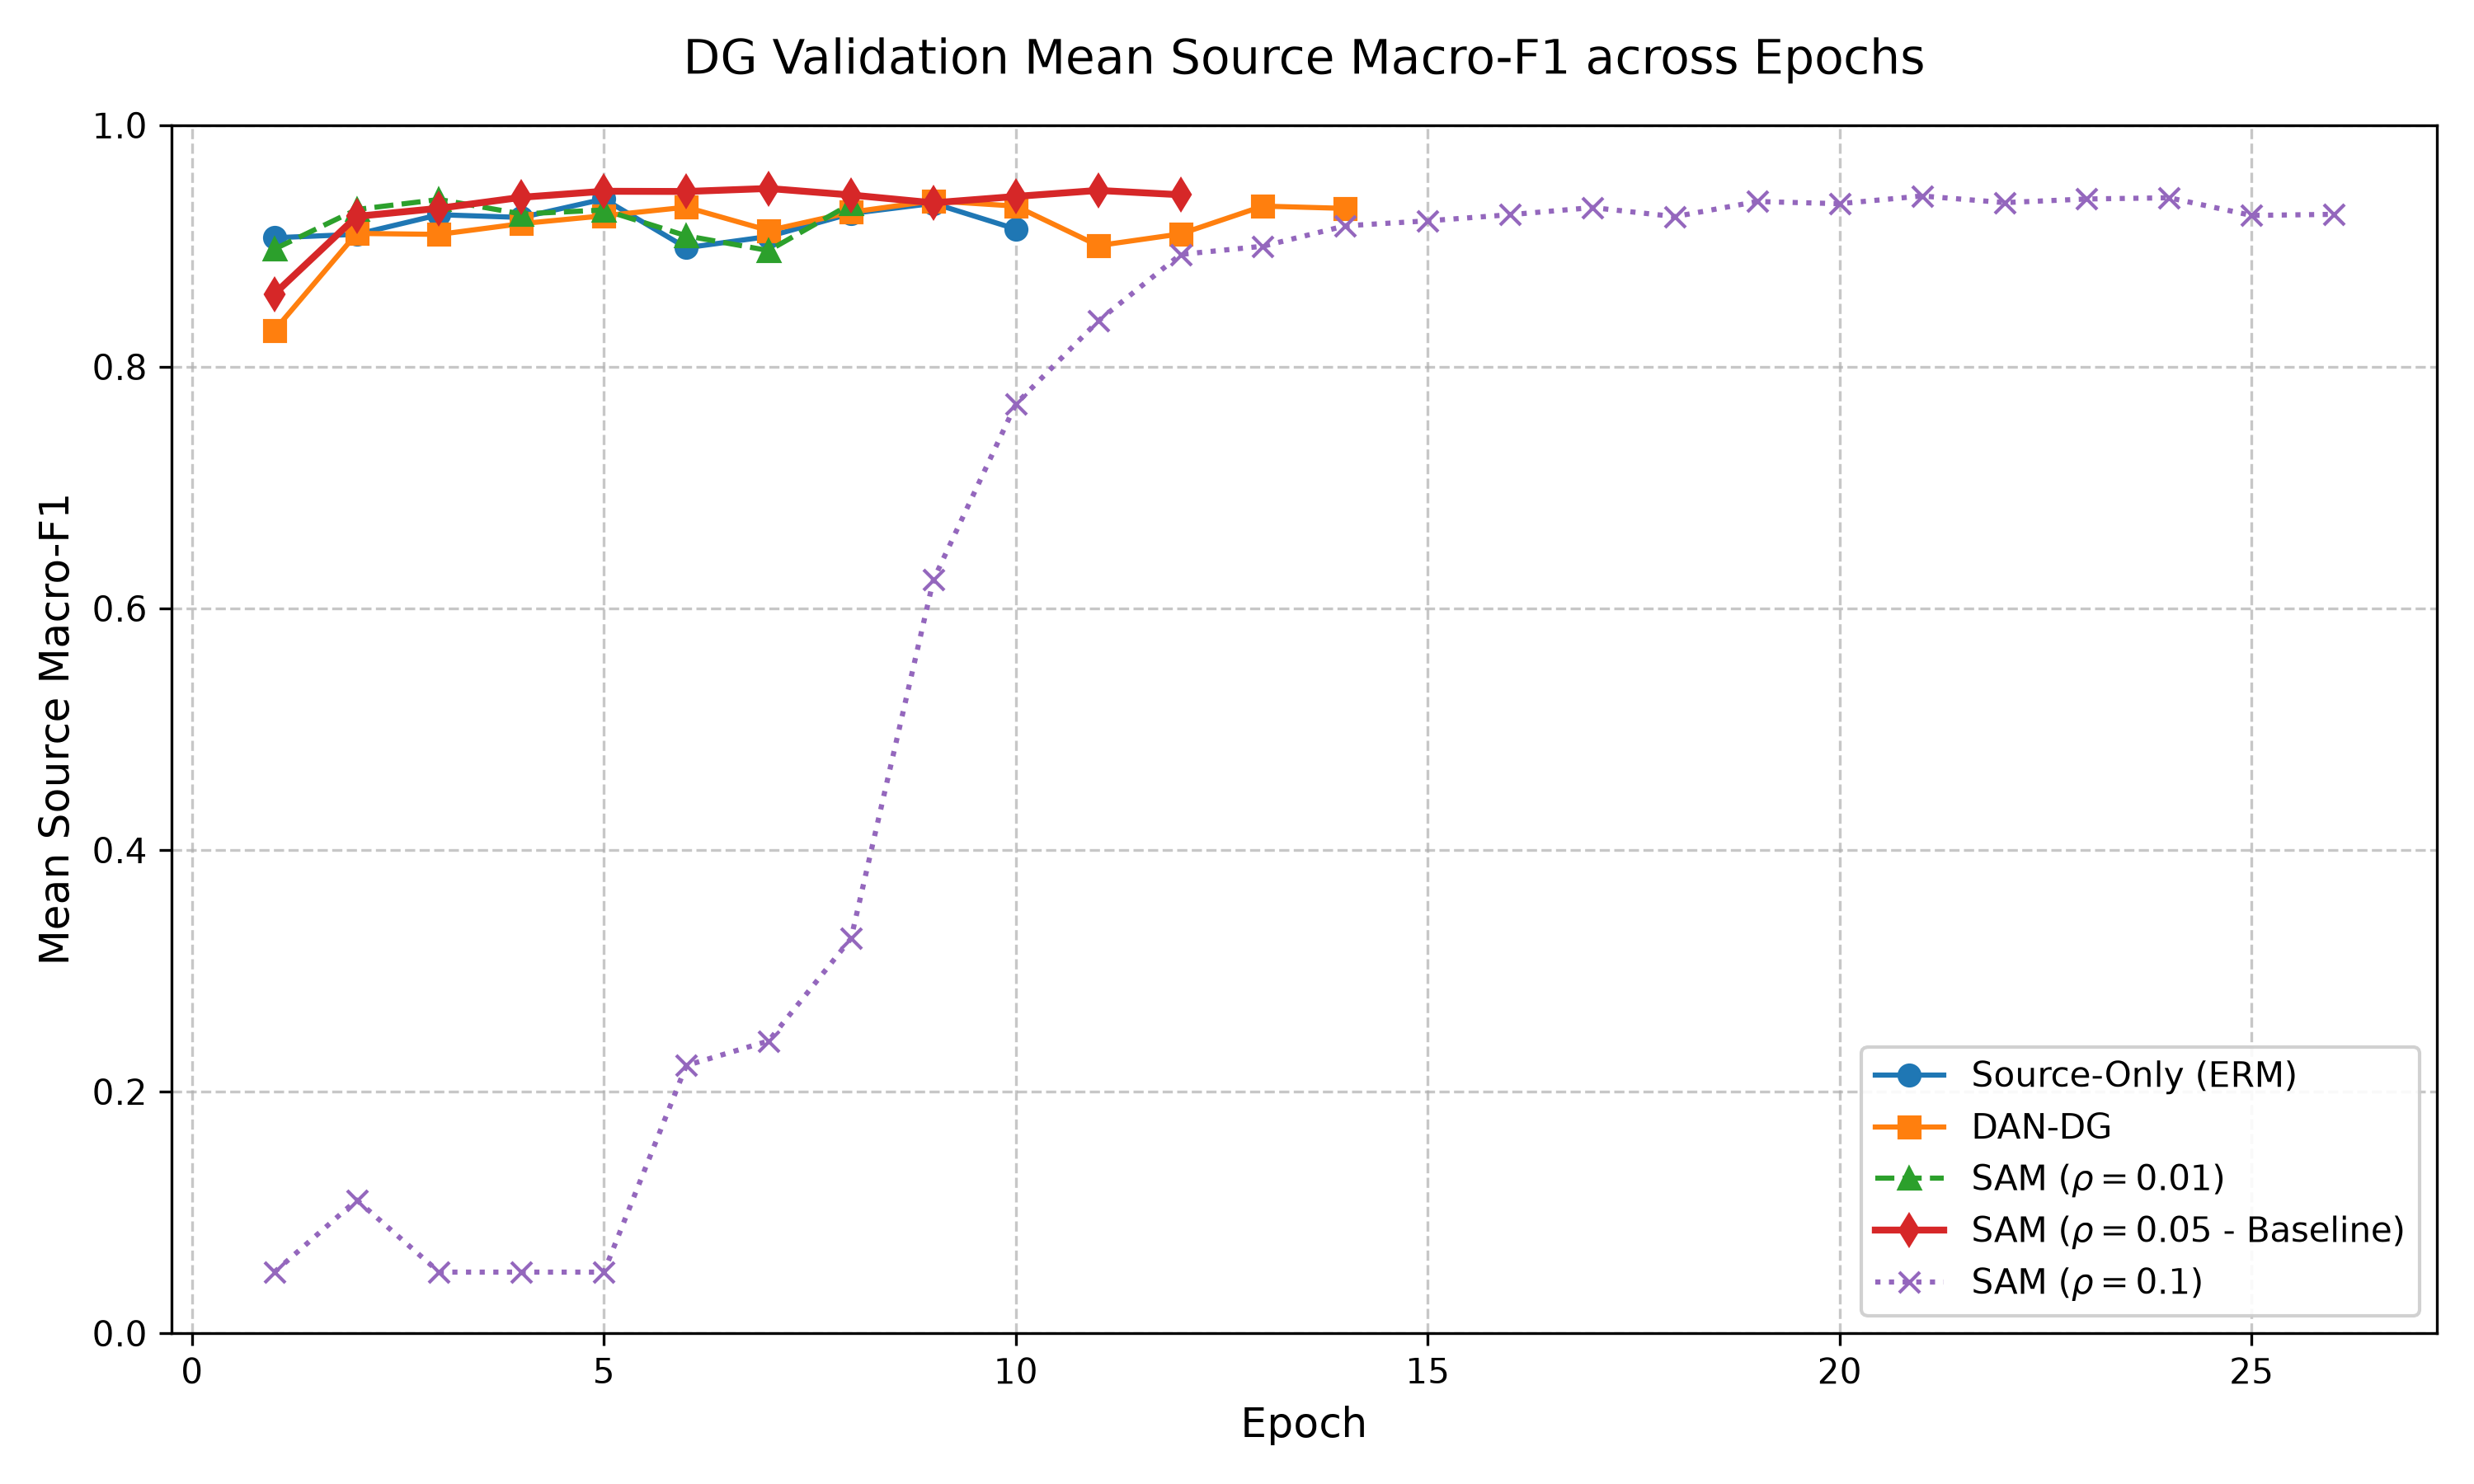
\includegraphics[width=0.8\textwidth]{../task3/results/training_curves.png}
  \caption{Validation Mean Source Macro-F1 across training epochs for the domain generalization paradigms. While ERM, DAN-DG, and baseline SAM converge smoothly, aggressively increasing the SAM perturbation radius ($\rho=0.1$) induces severe initial optimization instability before eventual recovery.}
  \label{fig:task3_training_curves}
\end{figure}

Figure~\ref{fig:task3_training_curves} illustrates the training trajectories for the generalization methods across the source validation sets. To prevent overfitting to the source domains, early stopping was enforced if the mean source-validation macro-F1 failed to improve for five consecutive epochs. The ERM baseline establishes a stable validation trajectory, hovering consistently above 0.90 macro-F1. DAN-DG similarly exhibits stable optimization, smoothly aligning the source domains without suffering the catastrophic feature collapse observed in target-aware adaptation, successfully triggering early stopping at epoch 14. 

The SAM optimization curves reveal a high sensitivity to the local perturbation radius constraint ($\rho$). At lower radii ($\rho=0.01$ and $\rho=0.05$), the model converges rapidly and stably, terminating at epochs 8 and 12, respectively, while achieving source validation scores marginally superior to the ERM baseline. However, aggressively expanding the neighborhood radius to $\rho=0.1$ causes immediate optimization failure. The initial ascent step pushes the parameters into a highly suboptimal region, plummeting the source macro-F1 to approximately 0.05 for the first five epochs. The model is eventually able to navigate out of this collapsed state, slowly recovering to a competitive validation score over 26 epochs. This trajectory underscores that while seeking flat minima can aid generalization, excessively large perturbation neighborhoods can temporarily destroy the pre-trained feature representations before the model re-converges.

\subsection{Task 4: OSR Training Trajectories and Optimization Diagnostics}
\label{appendix:task4_training}

To evaluate the capabilities of different Open-Set Recognition (OSR) frameworks, we strictly maintained a closed-set training environment consisting entirely of the ten CIFAR-10 known categories. All CIFAR-100 unknown evaluation images were withheld during all phases of training, representation learning, checkpoint selection, and hyperparameter tuning. Checkpoints for all models were selected exclusively based on the highest validation accuracy achieved on the CIFAR-10 known-class validation set.

All paradigms utilized a modified ResNet-18 architecture adapted for $32 \times 32$ spatial dimensions. The Vanilla baseline and GCSC models were trained from random initialization using Stochastic Gradient Descent (SGD) with a learning rate of 0.1, momentum of 0.9, and weight decay of $5 \times 10^{-4}$ subject to cosine decay over a strict 100-epoch budget. While the Vanilla model employed standard random crops and horizontal flipping, GCSC incorporated aggressive RandAugment operations (num\_ops=2, magnitude=9) to test the impact of improved closed-set generalization. 

PROSER was initialized from the optimal Vanilla checkpoint. It appended five dummy classifiers to the architecture and underwent fine-tuning for 50 epochs utilizing a reduced learning rate of $10^{-3}$. PROSER's batch optimization was divided: the first half of each batch minimized a classifier-placeholder loss on standard known images ($\beta=1$), while the second half minimized a data-placeholder loss ($\gamma=0.1$) on proxy-unknown representations generated via manifold mixup (sampled from a Beta(2, 2) distribution) applied between the second and third residual layers. Finally, the RPL extension replaced standard cross-entropy with a reciprocal point learning objective and an open-space regularization term to bound the known latent space, training from initialization for 100 epochs.

\begin{figure}[ht]
  \centering
  \begin{minipage}{0.48\textwidth}
    \centering
    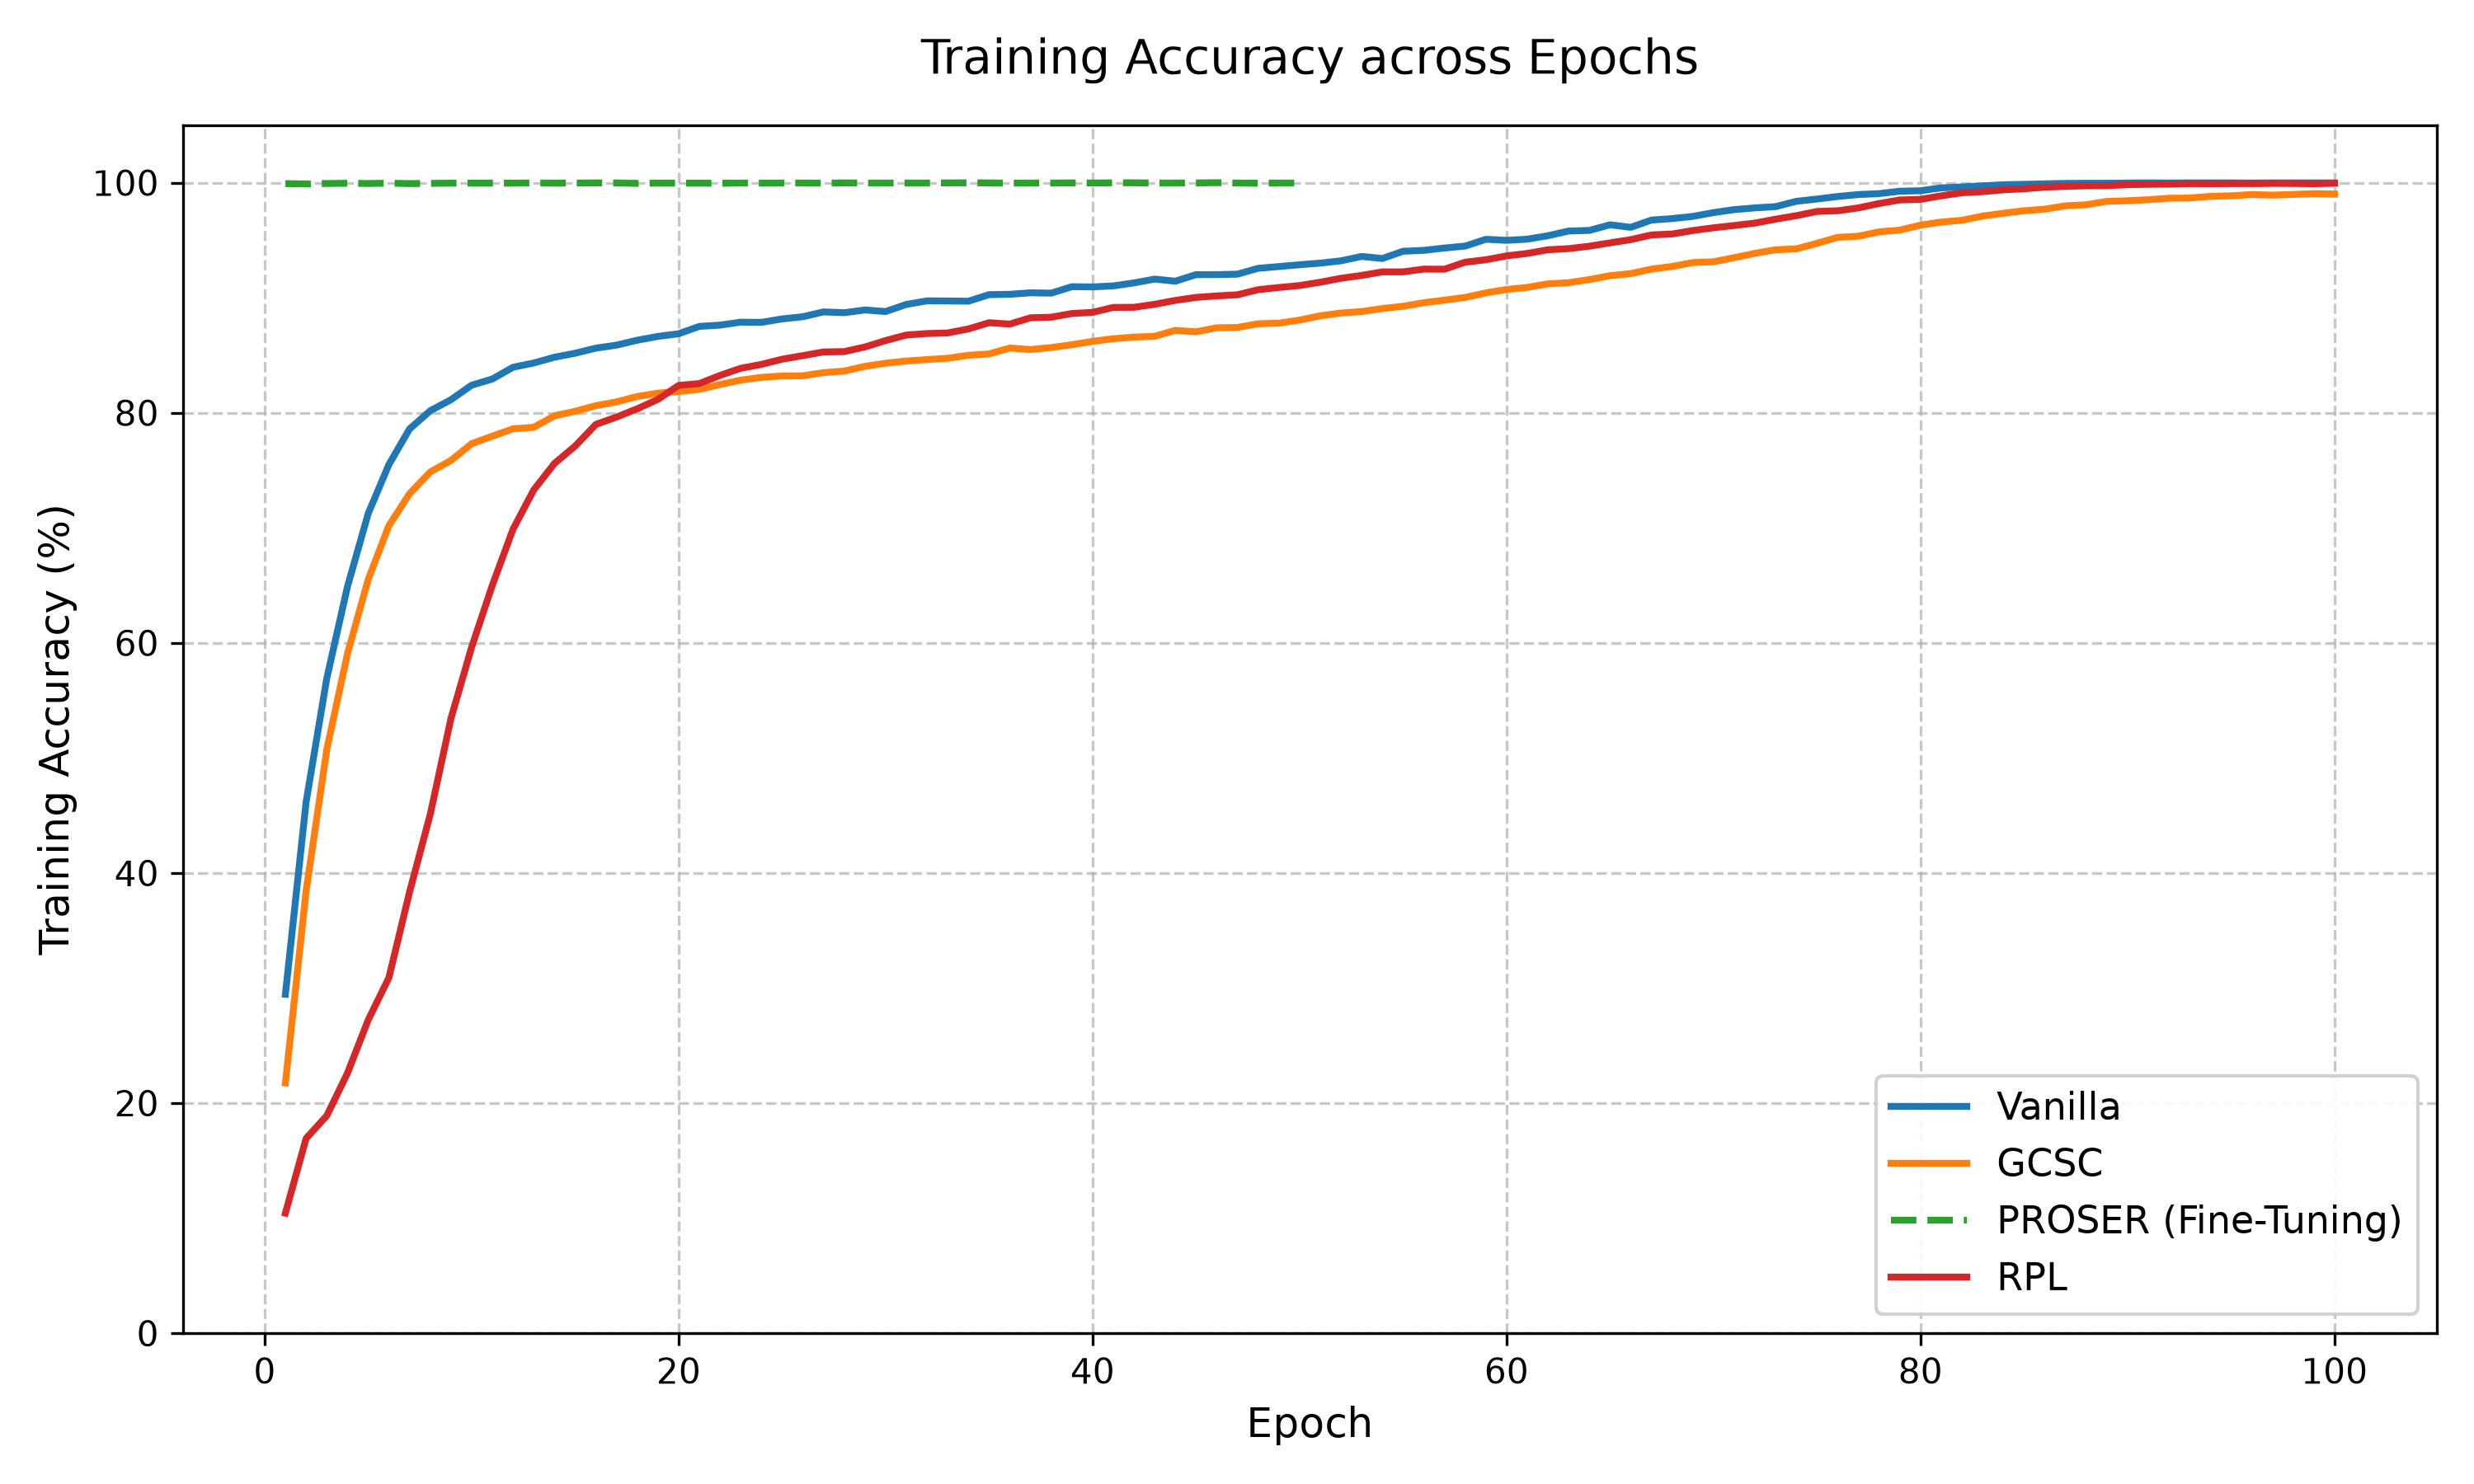
\includegraphics[width=\textwidth]{../task4/results/training_acc.png}
  \end{minipage}\hfill
  \begin{minipage}{0.48\textwidth}
    \centering
    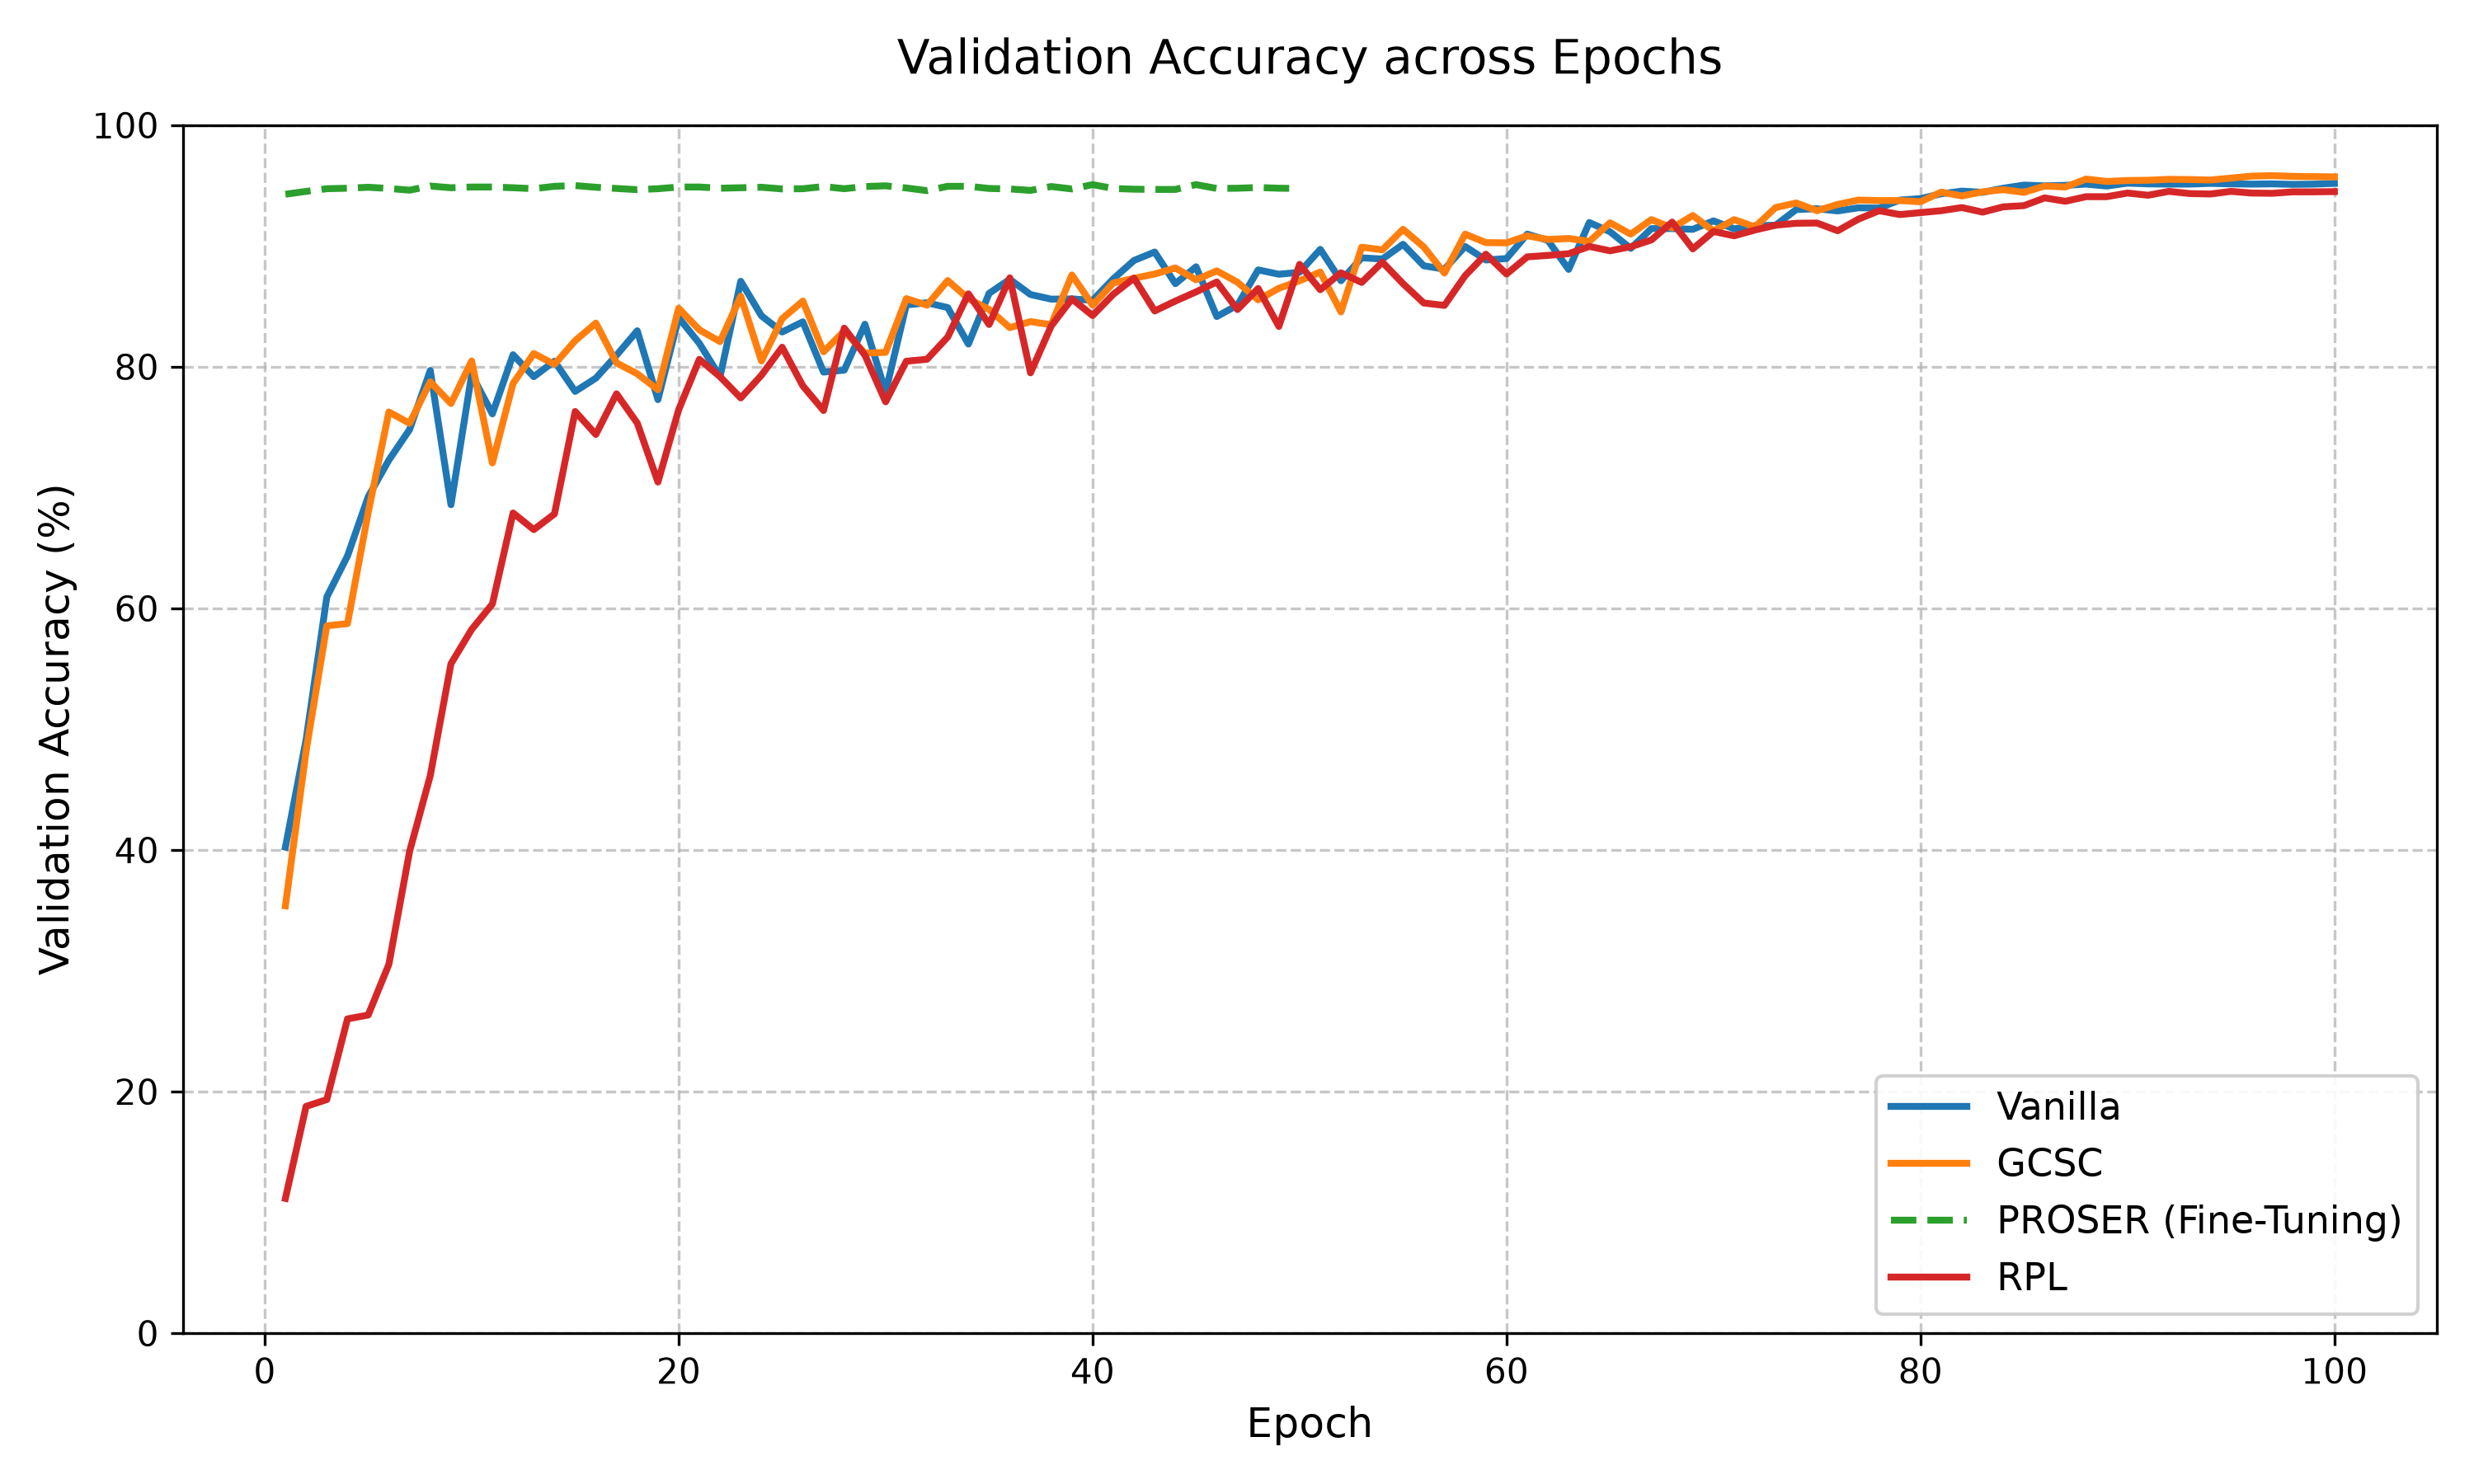
\includegraphics[width=\textwidth]{../task4/results/validation_acc.png}
  \end{minipage}
  \caption{Training (left) and validation (right) accuracy trajectories for the CIFAR-10 known-class optimization. Note that PROSER initializes from the pre-trained Vanilla checkpoint, resulting in near-perfect initial accuracy.}
  \label{fig:osr_training_curves}
\end{figure}

Figure~\ref{fig:osr_training_curves} illustrates the optimization trajectories for the evaluated paradigms. The Vanilla baseline converges rapidly, establishing strong in-distribution closed-set accuracy ($\sim$95\%). The injection of heavy spatial and color distortions in GCSC acts as a strong regularizer; while it suppresses training accuracy relative to the baseline, it successfully mitigates overfitting, ultimately yielding comparable or slightly superior validation performance. PROSER, initialized from the pre-trained Vanilla checkpoint, maintains near-perfect training accuracy and highly stable validation accuracy throughout its fine-tuning phase, indicating that the introduction of dummy classifiers and synthetic mixup placeholders does not catastrophically degrade the previously established known-class boundaries.

Conversely, RPL exhibits a significantly slower optimization trajectory compared to standard cross-entropy. Because RPL must learn explicit reciprocal anchors for every class and push representations away from them while simultaneously satisfying a bounding open-space constraint, the network requires the full 100-epoch budget to slowly force the latent space into this non-standard geometry, eventually reaching a competitive but slightly depressed validation accuracy ($\sim$94\%) relative to the Vanilla baseline.

\section{Feature Space Visualizations}
\label{appendix:tsne}

\begin{figure}[htbp]
  \centering
  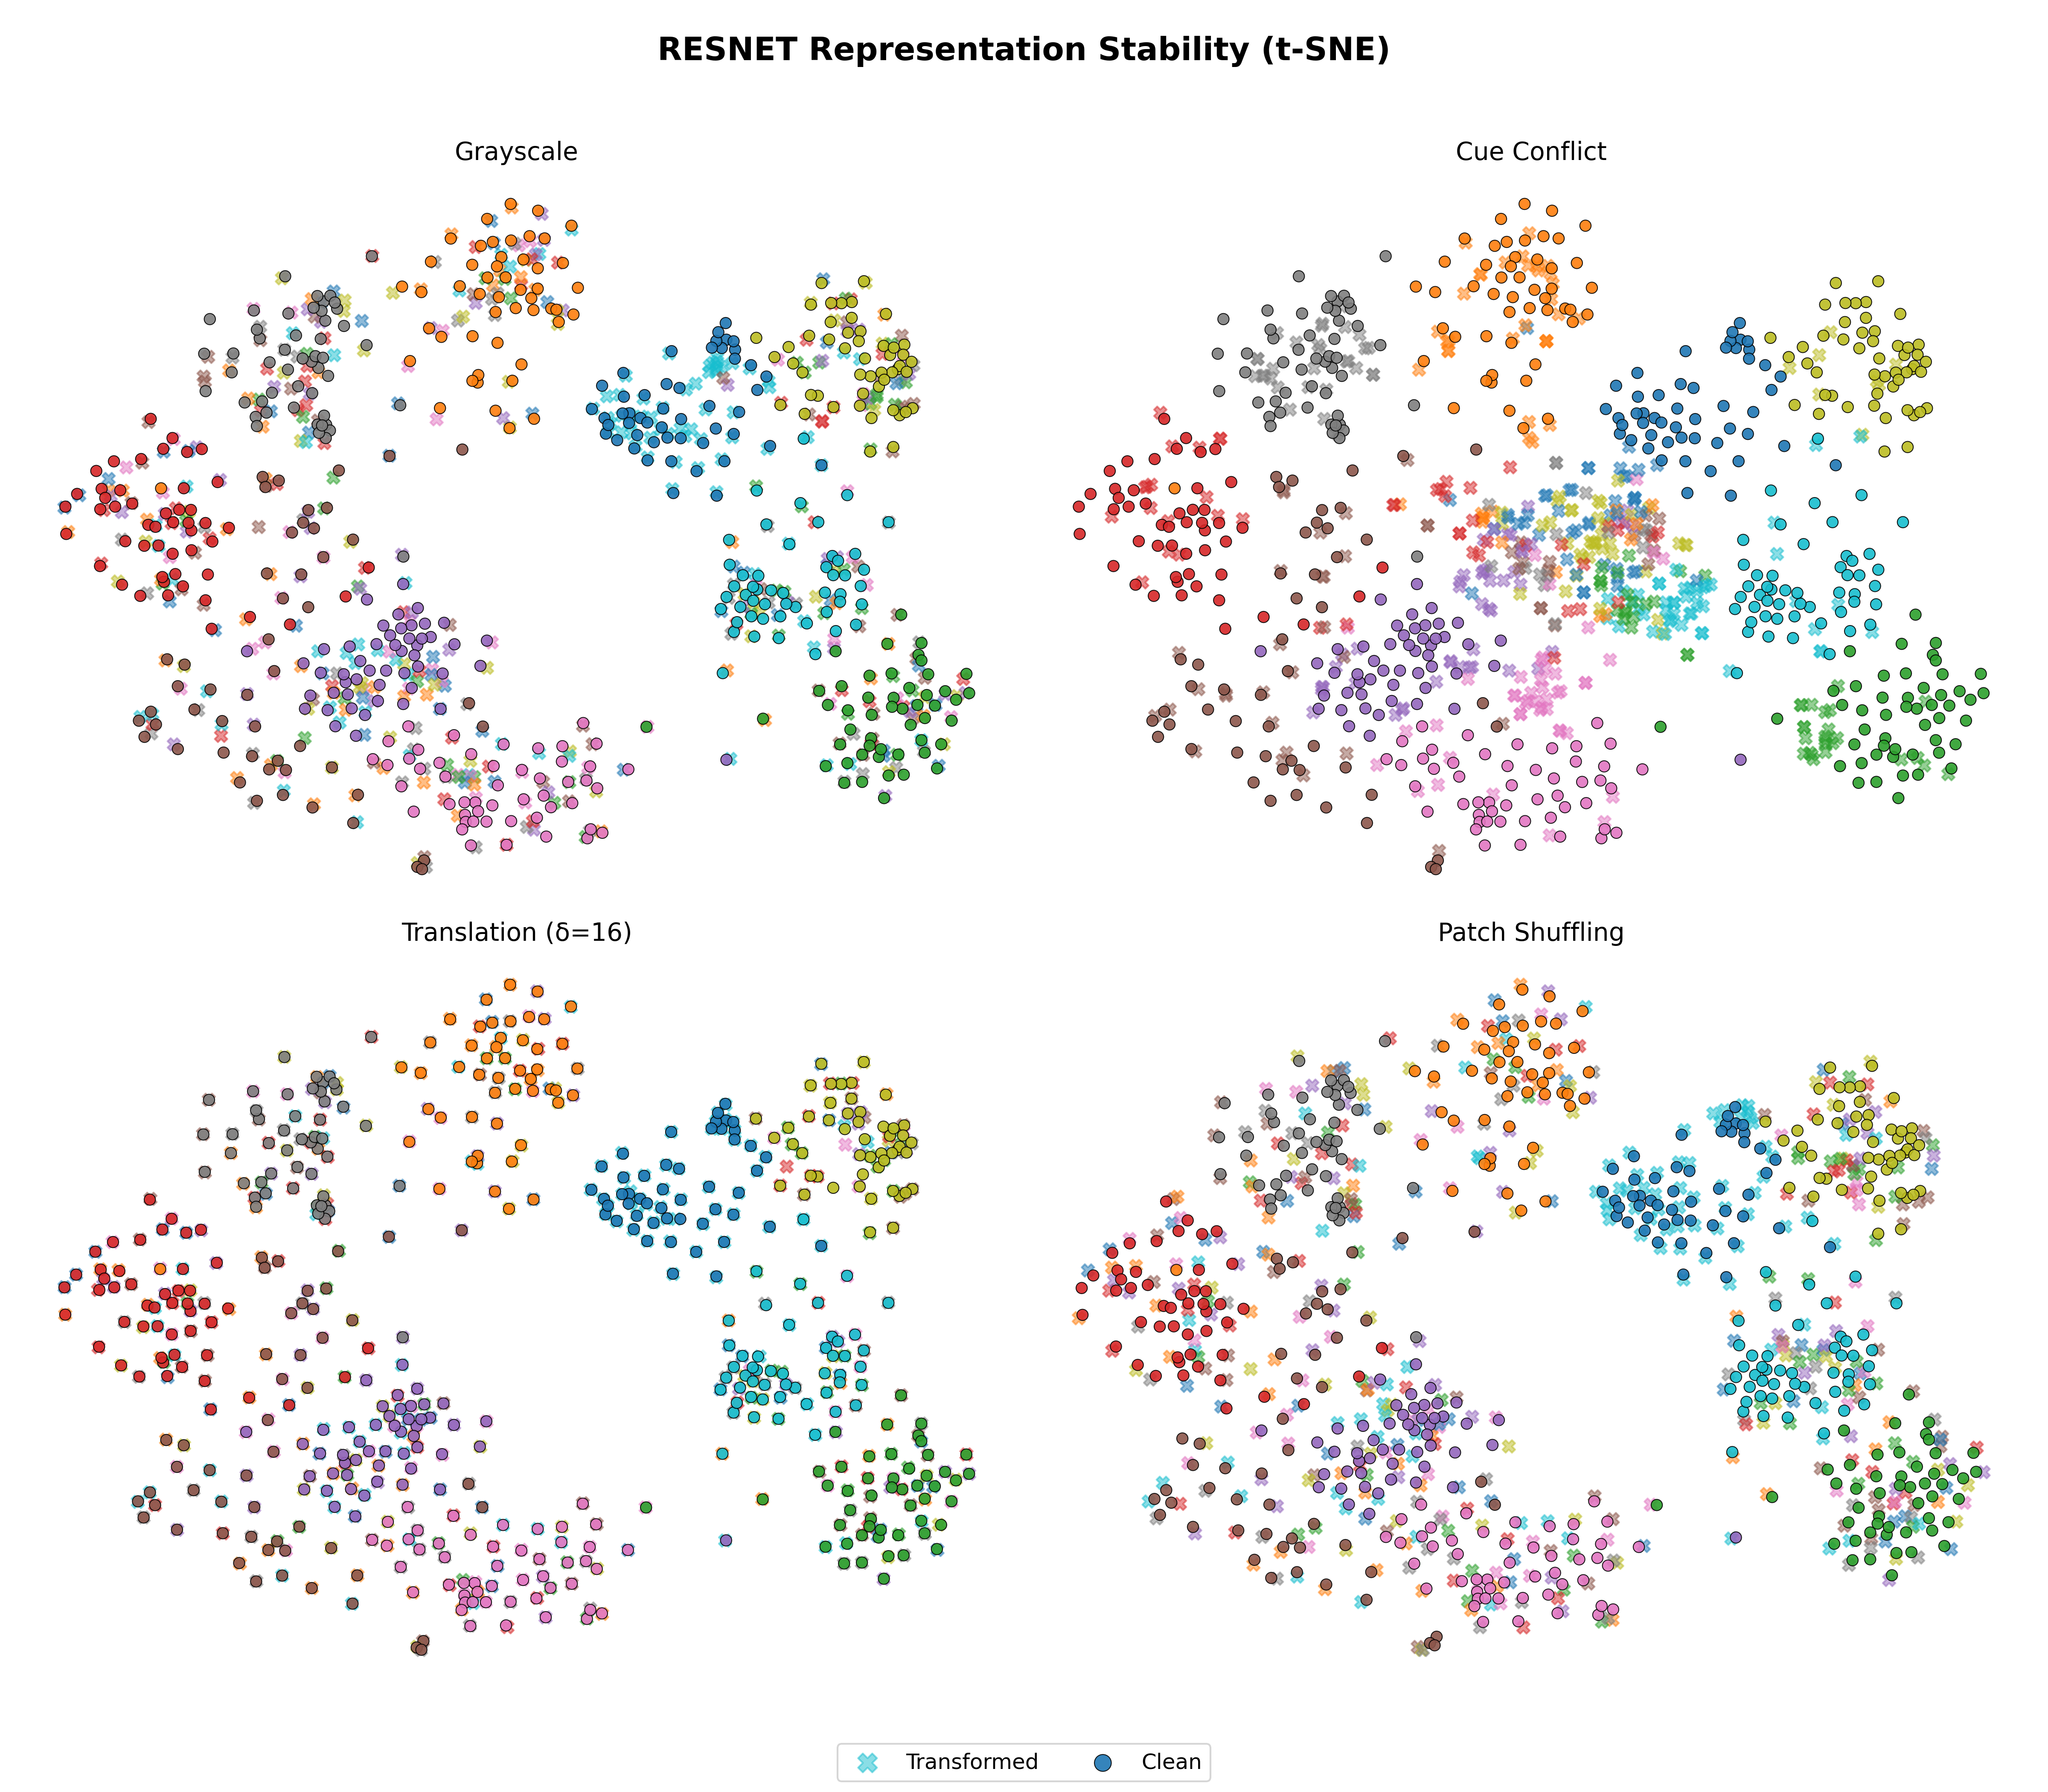
\includegraphics[width=0.9\textwidth]{../task1/results/resnet_tsne.png}
  \caption{Two-dimensional t-SNE projections comparing clean and transformed latent representations for ResNet-50. Despite the model maintaining stable predictions under cue-conflict transformations, the plotted representations shift drastically from their clean counterparts, revealing a mismatch between feature stability and final classification.}
\end{figure}

\begin{figure}[htbp]
  \centering
  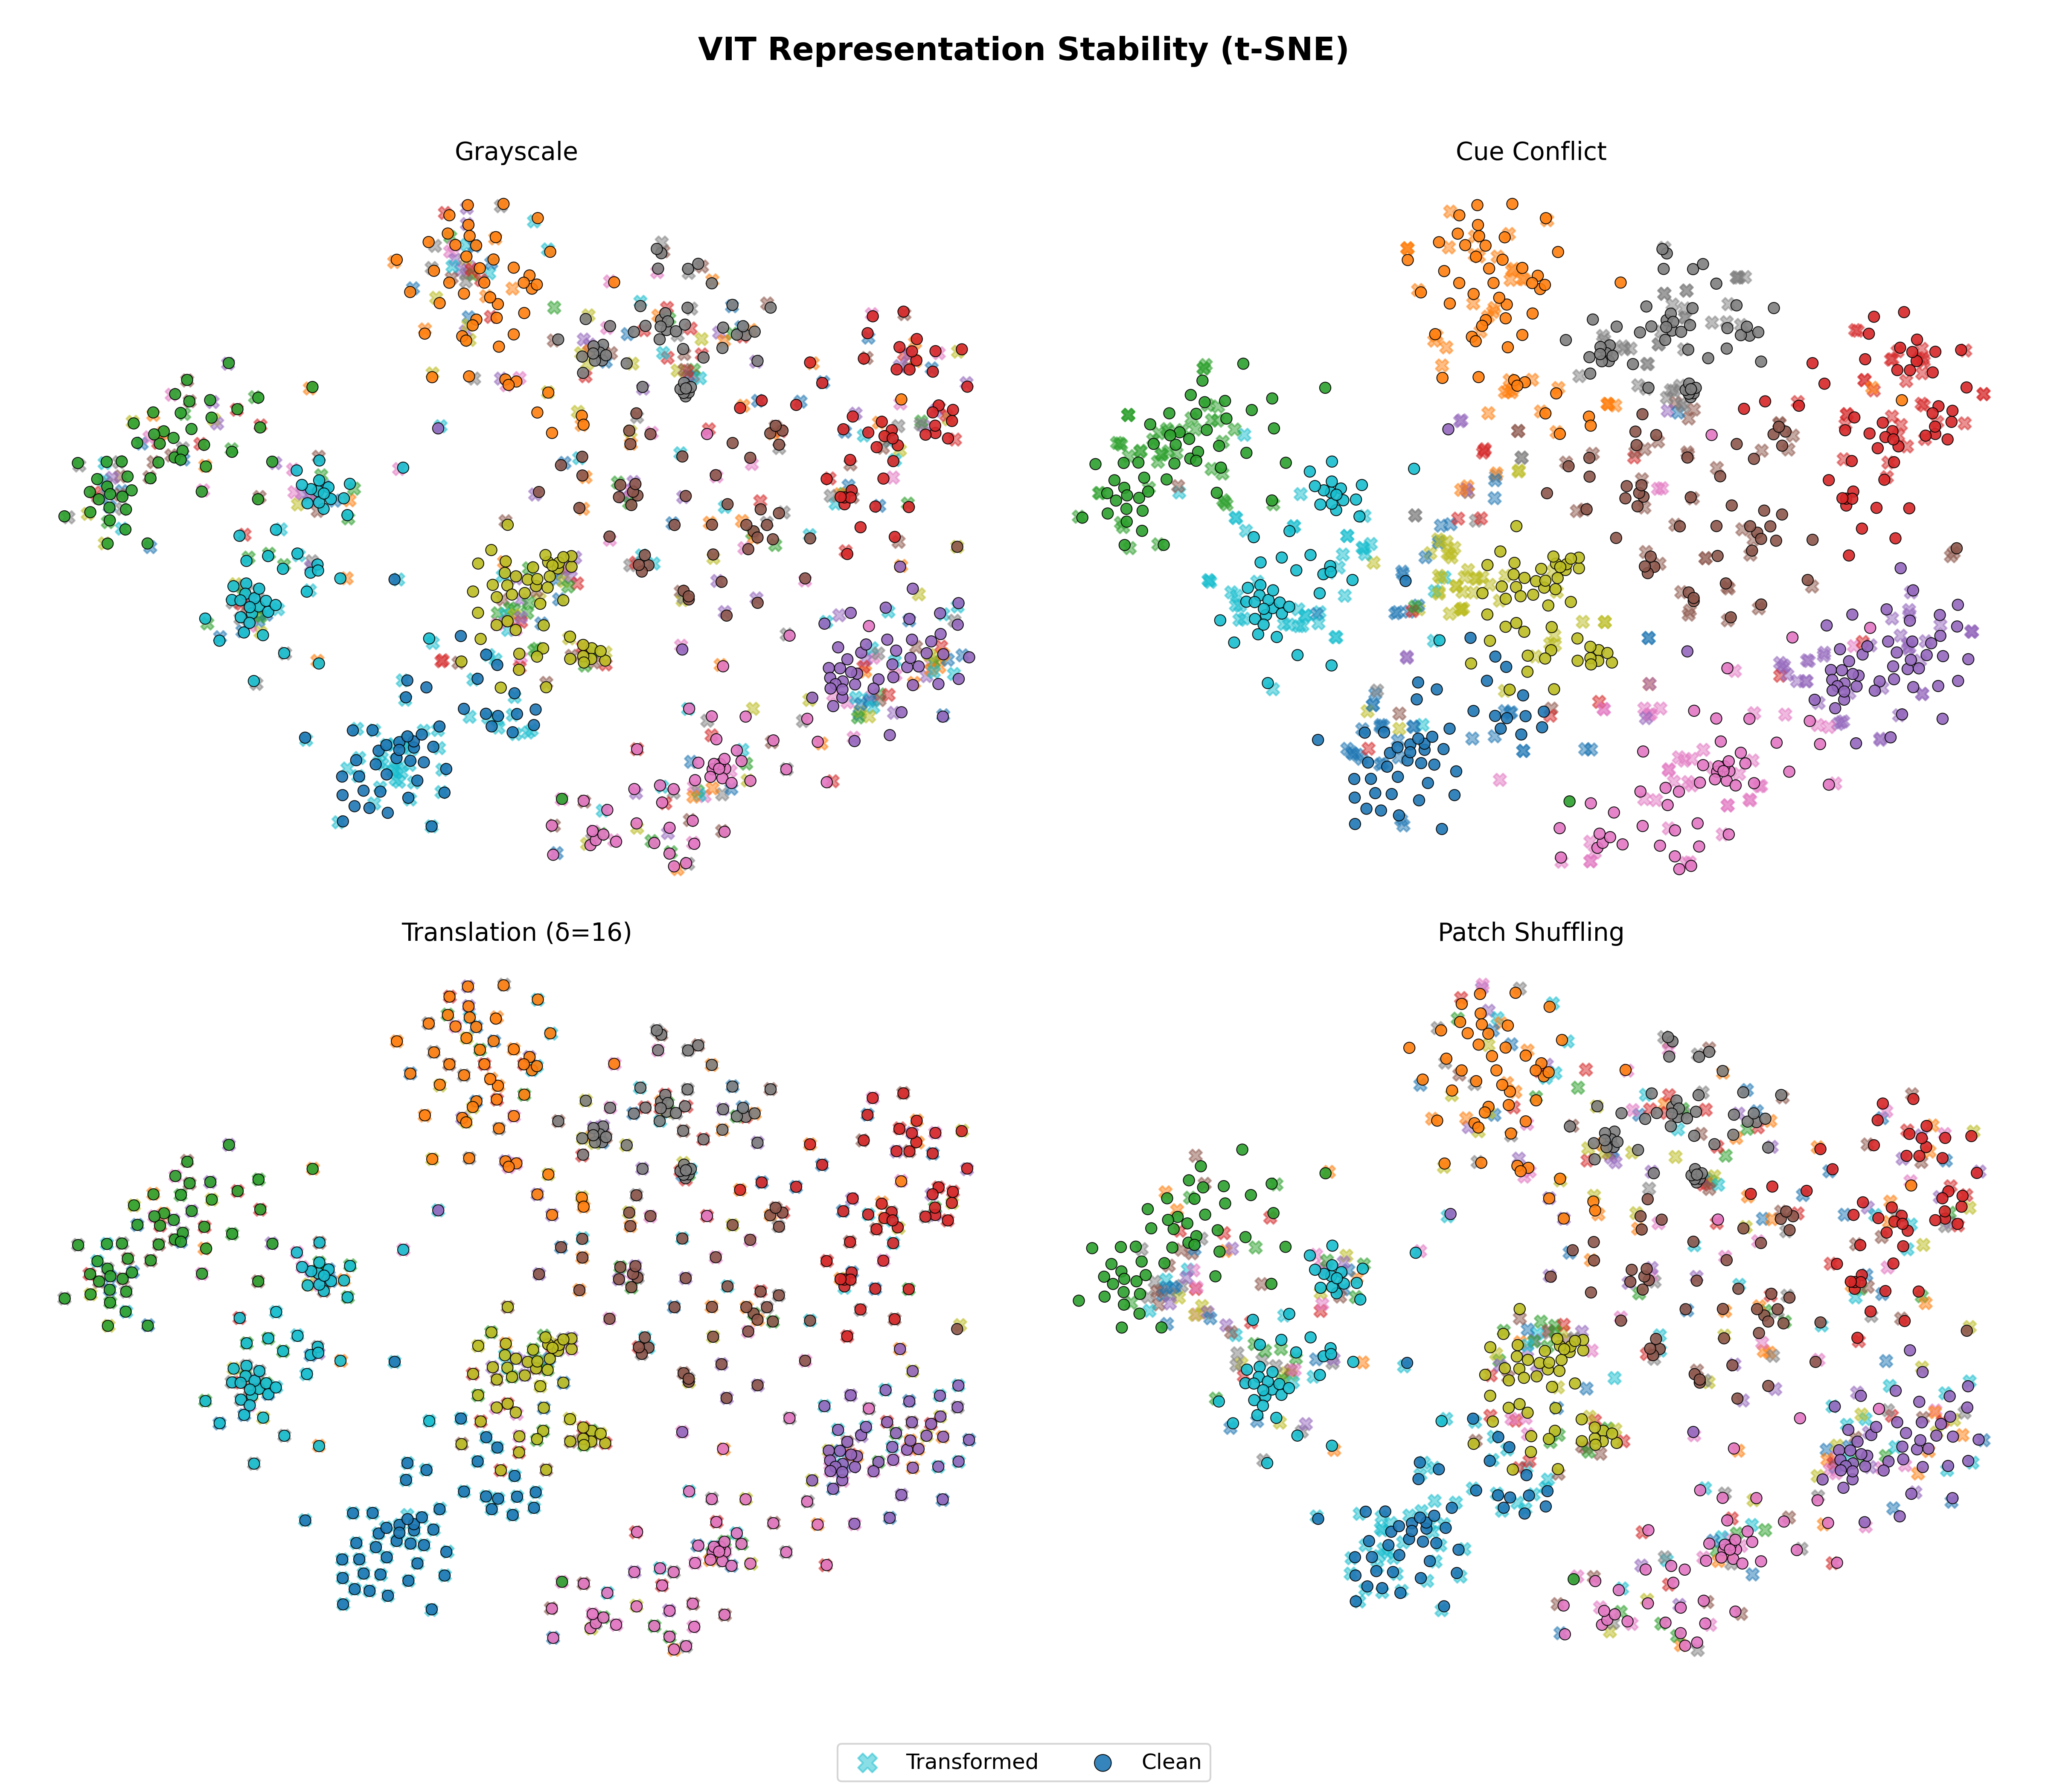
\includegraphics[width=0.9\textwidth]{../task1/results/vit_tsne.png}
  \caption{Two-dimensional t-SNE projections comparing clean and transformed latent representations for ViT-B/16. The transformer representations also undergo a drift under cue conflicts. However, unlike the convolutional baseline, the drift still manages to keep the representations near the clean latent representations.}
\end{figure}

\begin{figure}[htbp]
  \centering
  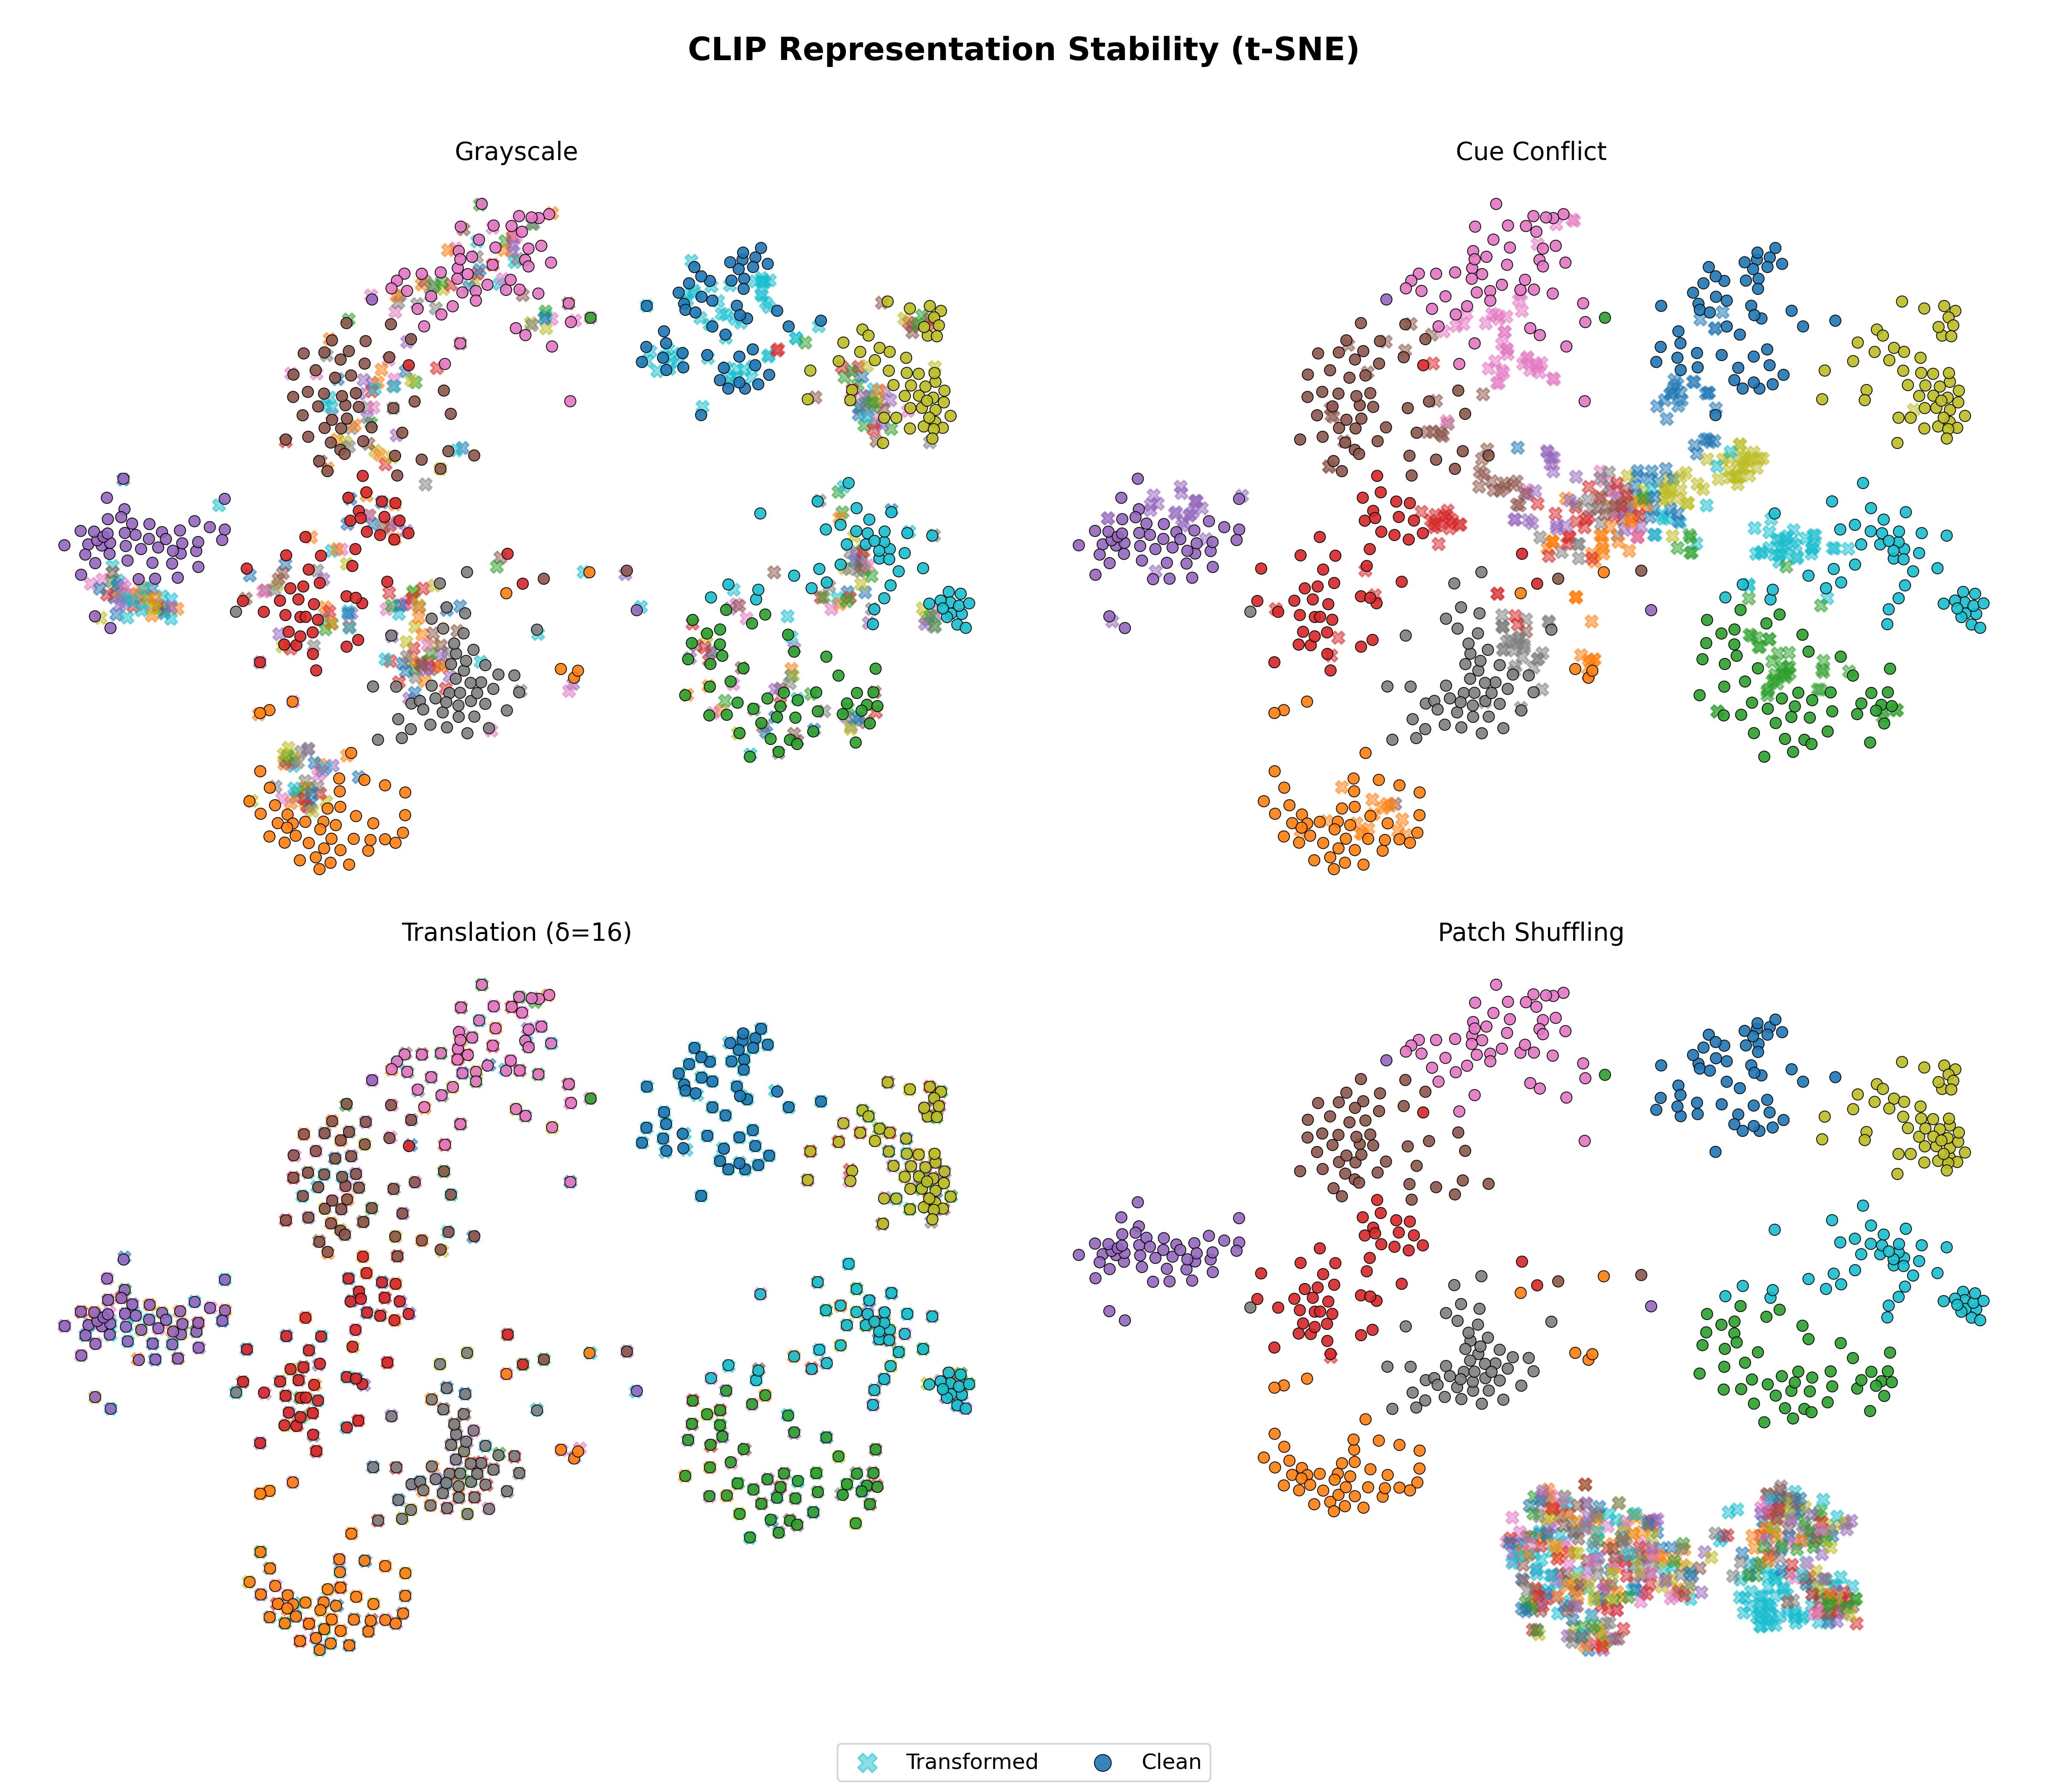
\includegraphics[width=0.9\textwidth]{../task1/results/clip_tsne.png}
  \caption{Two-dimensional t-SNE projections comparing clean and transformed latent representations for CLIP. Crucially, the patch-shuffled inputs collapse into a single, isolated, non-discriminative group in the bottom corner, demonstrating that preserving the raw visual tokens without spatial coherence destroys class separability.}
\end{figure}

\end{document}
